\documentclass[journal]{IEEEtran}
% \documentclass[journal,12pt,onecolumn,draftclsnofoot]{IEEEtran}

\usepackage[table]{xcolor}
\usepackage{adjustbox}
\usepackage{algorithm}
\usepackage{algpseudocode}
\usepackage{amsfonts}
\usepackage{amsmath}
\usepackage{amssymb}
\usepackage{amsthm}
\usepackage{bookmark}
\usepackage{booktabs}
\usepackage[makeroom]{cancel}
\usepackage[american]{circuitikz}
\usepackage{cite}
\usepackage{fixmath}
\usepackage[acronym]{glossaries-extra}
\usepackage{hyperref}
\usepackage{import}
\usepackage{mathtools}
\usepackage{microtype}
\usepackage[short]{optidef}
\usepackage{pgfplots}
\usepackage{ragged2e}
\usepackage[subtle]{savetrees}
\usepackage{siunitx}
\usepackage{stfloats}
\usepackage[caption=false,font=footnotesize,subrefformat=parens,labelformat=parens]{subfig}
\usepackage{tabularx}
\usepackage{tikz}
\usepackage{graphicx}
\usepackage{epstopdf}

% page limit hacks
% \usepackage{setspace}
% ! \usepackage[top=1cm, bottom=1cm, left=1cm, right=1cm]{geometry}
% \abovedisplayskip=1mm
% \belowdisplayskip=1mm
% \abovedisplayshortskip=1mm
% \belowdisplayshortskip=1mm
% \setlength{\jot}{0.1mm}
% \setlength{\floatsep}{1mm}
% \setlength{\textfloatsep}{1mm}
% \setlength{\intextsep}{1mm}
% \setlength{\skip\footins}{2mm}


% amsthm
\newtheorem{proposition}{Proposition}
\newtheorem{remark}{Remark}

% PGF/TikZ
\usetikzlibrary{arrows,calc,matrix,patterns,plotmarks,positioning,shapes}
\usetikzlibrary{decorations.pathmorphing,decorations.pathreplacing,decorations.shapes,shapes.geometric}
\usepgfplotslibrary{groupplots,patchplots}
\pgfplotsset{compat=newest}

% tabularx, ragged2e
\newcolumntype{L}{>{\RaggedRight}X}
\newcolumntype{C}{>{\centering\arraybackslash}X}
\renewcommand\tabularxcolumn[1]{m{#1}}

% algpseudocode
\makeatletter
\renewcommand{\fnum@algorithm}{\fname@algorithm{} \thealgorithm:}
\newcommand\setalgorithmcaptionfont[1]{%
	\let\my@floatc@ruled\floatc@ruled          % save \floatc@ruled
	\def\floatc@ruled{%
		\global\let\floatc@ruled\my@floatc@ruled % restore \floatc@ruled
		#1\floatc@ruled}}
\makeatother

\algrenewcommand{\algorithmicrequire}{\textbf{Input:}}
\algrenewcommand{\algorithmicensure}{\textbf{Output:}}
\algrenewcommand{\algorithmicwhile}{\textbf{While}}
\algrenewcommand{\algorithmicend}{\textbf{End}}
\algrenewcommand{\algorithmicrepeat}{\textbf{Repeat}}
\algrenewcommand{\algorithmicuntil}{\textbf{Until}}
\algrenewcommand{\algorithmicfor}{\textbf{For}}
\algrenewcommand{\algorithmicdo}{}

% optidef
\DeclareDocumentEnvironment{customopti}{D||{\defaultProblemFormat} O{\defaultConstraintFormat} D<>{} m m m m m}{%
	\ifthenelse{\equal{#3}{b}}{%
		\ifthenelse{\equal{#1}{s}}%
		% Short version problem
		{\setFormatShort{#4}{#5}\BaseMiniStar{#2}{#5}{#6}{#8}{#4}{#3}}%
		% Long version problem
		{\setFormatLong{#4}{#5}\BaseMiniStar{#2}{#5}{#6}{#8}{#4}{#3}}%
	}{%
		\ifthenelse{\equal{#1}{s}}%
		% Short version problem
		{\setFormatShort{#4}{#5}\BaseMini{#2}{#5}{#6}{#7}{#8}{#4}}%
		% Long version problem
		{\setFormatLong{#4}{#5}\BaseMini{#2}{#5}{#6}{#7}{#8}{#4}}%
	}%
}%
{\endBaseMini\toggletrue{bodyCon}}

\DeclareDocumentEnvironment{customopti*}{D||{\defaultProblemFormat} O{\defaultConstraintFormat} D<>{} m m m m m}{%
	\ifthenelse{\equal{#1}{s}}%
	% Short version problem
	{\setFormatShort{#4}{#5}\BaseMiniStar{#2}{#5}{#6}{#8}{#4}{#3}}%
	% Long version problem
	{\setFormatLong{#4}{#5}\BaseMiniStar{#2}{#5}{#6}{#8}{#4}{#3}}%
}{\endBaseMiniStar\toggletrue{bodyCon}}

\DeclareDocumentEnvironment{customopti!}{D||{\defaultProblemFormat} O{\defaultConstraintFormat} D<>{} m m m m m}{%
	\ifthenelse{\equal{#1}{s}}%
	% Short version problem
	{\setFormatShort{#4}{#5}\BaseMiniExclam{#2}{#5}{#6}{#7}{#8}{#4}{#3}}%
	% Long version problem
	{\setFormatLong{#4}{#5}\BaseMiniExclam{#2}{#5}{#6}{#7}{#8}{#4}{#3}}%
}{\endBaseMiniExclam\toggletrue{bodyCon}}

% glossaries-extra
\glsdisablehyper
\setabbreviationstyle[acronym]{long-short}
\newacronym{ao}{AO}{Alternating Optimization}
\newacronym{bd}{BD}{Beyond-Diagonal}
\newacronym{bcd}{BCD}{Block Coordinate Descent}
\newacronym{dof}{DoF}{Degree of Freedom}
\newacronym{siso}{SISO}{Single-Input Single-Output}
\newacronym{miso}{MISO}{Multiple-Input Single-Output}
\newacronym{mimo}{MIMO}{Multiple-Input Multiple-Output}
\newacronym{rcg}{RCG}{Riemannian Conjugate Gradient}
\newacronym{ris}{RIS}{Reconfigurable Intelligent Surface}
\newacronym{pc}{PC}{Point-to-point Channel}
\newacronym{ic}{IC}{Interference Channel}
\newacronym{snr}{SNR}{Signal-to-Noise Ratio}
\newacronym{wsr}{WSR}{Weighted Sum-Rate}
\newacronym{svd}{SVD}{Singular Value Decomposition}
\newacronym{mmse}{MMSE}{Minimum Mean-Square Error}
\newacronym{wmmse}{WMMSE}{Weighted \gls{mmse}}
\newacronym{mse}{MSE}{Mean-Square Error}
\newacronym{los}{LoS}{Line-of-Sight}
\newacronym{csi}{CSI}{Channel State Information}
\newacronym{cscg}{CSCG}{Circularly Symmetric Complex Gaussian}


\begin{document}
\title{Channel Shaping Using Reconfigurable Intelligent Surfaces: From Diagonal to Beyond}
\author{
	\IEEEauthorblockN{
		Yang~Zhao,~\IEEEmembership{Member,~IEEE,}
		Hongyu~Li,~\IEEEmembership{Graduate Student Member,~IEEE,}\\
		Massimo~Franceschetti,~\IEEEmembership{Fellow,~IEEE,}
		and~Bruno~Clerckx,~\IEEEmembership{Fellow,~IEEE}
	}
	% \thanks{
	% 	The authors are with the Department of Electrical and Electronic Engineering, Imperial College London, London SW7 2AZ, U.K. (e-mail: \{yang.zhao18, b.clerckx\}@imperial.ac.uk).
	% 	B. Clerckx is also with Silicon Austria Labs (SAL), Graz A-8010, Austria.
	% }
}
\maketitle

\begin{abstract}
	This paper investigates how a passive \gls{ris} can reshape the \gls{mimo} point-to-point channel in terms of singular values.
	We depart from the widely-adapted diagonal phase shift model to a general \gls{bd} architecture, which provides superior shaping capability thanks to in-group connections between elements.
	An efficient \gls{rcg} algorithm is tailored for smooth optimization problems of asymmetric \gls{bd}-\gls{ris} with arbitrary group size, then invoked for the Pareto frontier of channel singular values.
	To understand the gain from off-diagonal entries, we also derive analytical singular value bounds in \gls{los} and fully-connected scenarios.
	As a side product, we tackle \gls{mimo} rate maximization problem by alternating between active beamformer (eigenmode transmission) and passive beamformer (\gls{rcg} algorithm) until convergence.
	A low-complexity suboptimal solution based on channel shaping is also proposed, where the decoupled problem is formulated as channel power maximization and solved in closed form iteratively.
	% We then show how channel shaping decouples the design and amounts to a low-complexity suboptimal solution.
	% A low-complexity suboptimal solution decoupling both blocks is also proposed, where the channel shaping subproblem is formulated as channel power maximization and solved in closed form iteratively.
	Theoretical analysis and numerical evaluation reveal that the shaping advantage of \gls{bd}-\gls{ris} increases with group size and \gls{mimo} dimensions, stemming from stronger subchannel rearrangement and subspace alignment capabilities.
\end{abstract}

\begin{IEEEkeywords}
	Reconfigurable intelligent surface, multi-input multi-output, manifold optimization, singular value control, rate maximization.
\end{IEEEkeywords}

\glsresetall

\begin{section}{Introduction}
	% The quest for reliable, high-speed, and ubiquitous wireless connectivity has been long-standing since Marconi's illuminating radio in 1895.
	% Great successes have been made at transmitter and receiver sides over the past century, and the society is unprecedentedly close to the Shannon limit \cite{Shannon1948}.
	Today we are witnessing a paradigm shift from connectivity to intelligence, where the wireless environment is no longer a chaotic medium but a conscious agent that serves on demand.
	This is empowered by the recent advances in \gls{ris}, a real-time programmable metasurface of numerous non-resonant sub-wavelength scattering elements.
	It can manipulate the amplitude, phase, frequency, and polarization of the scattered waves \cite{Basar2019} with a higher energy efficiency, lower cost, lighter footprint, and greater scalability than relays.
	Using \gls{ris} for {passive beamforming} has attracted significant interest in wireless communication \cite{Wu2019,Wu2020c,Yang2020,Zheng2021}, backscatter \cite{Jia2020,Liang2022}, sensing \cite{Liu2022a,Hua2023}, and power transfer literature \cite{Wu2021d,Feng2022,Zhao2022}, reporting a second-order array gain and fourth-order power scaling law (with proper waveform).
	On the other hand, \gls{ris} also enables {backscatter modulation} by dynamically switching between different patterns, as already investigated \cite{Karasik2020,Basar2020,Zhao2022a} and prototyped \cite{Tang2019a,Dai2020a}.
	Despite fruitful outcomes, one critical unanswered question is the {channel shaping} capability: \emph{To what extent can a passive \gls{ris} reshape the wireless channel?}

	The answer indeed depends on the hardware architecture and scattering model.
	In conventional (a.k.a. diagonal) \gls{ris}, each scattering element is tuned by a dedicated impedance and acts as an \emph{individual} phase shifter \cite{Wu2020}.
	The concept is generalized to \gls{bd}-\gls{ris} \cite{Shen2020a,Li2023b} which groups adjacent elements using passive components.
	This allows \emph{cooperative} scattering --- wave impinging on one element can propagate within the circuit and depart partially from any element in the same group.
	\gls{bd}-\gls{ris} can thus control both amplitude and phase of the reflected wave, generalizing the scattering matrix from diagonal with unit-magnitude entries to block diagonal with  unitary blocks.
	Its benefit has been recently shown in receive power maximization \cite{Nerini2023,Santamaria2023,Fang2023,Nerini2023a}, transmit power minimization \cite{Zhou2023}, and rate maximization \cite{Zhou2023,Nerini2023a,Li2023d,Bartoli2023,Li2023c}.
	Practical issues such as channel estimation \cite{Li2023e} and mutual coupling \cite{Li2023f} have also been investigated.
	Therefore, \gls{bd}-\gls{ris} is envisioned as the next generation channel shaper with stronger signal processing flexibility \cite{Li2023g}.

	% Attempts to characterize the channel shaping capability can be classified into \emph{singular value centric} and \emph{power centric} methods.
	% Channel shaping is different from passive beamforming as it seeks to modify the inherent properties of the channel itself, allowing one to decouple \gls{ris} and transceiver design.
	Channel shaping is different from passive beamforming as it seeks to modify the inherent properties of the channel itself.
	This allows one to decouple the \gls{ris}-transceiver design and explore the fundamental limits of channel manipulation.
	For example, diagonal \gls{ris} has been proved useful for improving channel power \cite{Ning2020}, degree of freedom \cite{Ozdogan2020,Li2023h}, condition number \cite{Zheng2022,Huang2023}, and effective rank \cite{ElMossallamy2021,Meng2023} in \gls{mimo}.
	In contrast, \gls{bd}-\gls{ris} can provide a higher channel power but existing results are limited to \gls{siso}\footnote{In terms of channel shaping, single-stream \gls{mimo} with given precoder and combiner \cite{Nerini2023} is equivalent to \gls{siso}.}. \cite{Nerini2023} and \gls{miso} \cite{Santamaria2023}.
	While these studies offer promising glimpses into the channel shaping potential, a comprehensive understanding of the capabilities and limitations is desired, and a universal design framework is missing.
	This paper aims to answer the channel shaping question through theoretical analysis and numerical optimization.
	The contributions are summarized below.

	First, we quantify the capability of a \gls{bd}-\gls{ris} to reshape the \gls{mimo} point-to-point channel in terms of singular values.
	The \emph{Pareto frontiers} are characterized by optimizing the {weighted sum of singular values}, where the weights can be positive, zero, or negative.
	% This generalizes most singular value metrics and provides a powerful design framework.
	The resulting region generalizes most relevant metrics and provides an intuitive channel shaping benchmark.
	We then discuss some analytical singular value bounds in \gls{los} and fully-connected scenarios, which help to demystify the gain from off-diagonal entries.
	This is the first paper to answer the channel shaping question and highlight the \gls{bd}-\gls{ris} gain from a Pareto perspective.

	Second, we propose a \gls{rcg} algorithm for smooth optimization problems of asymmetric \gls{bd}-\gls{ris} with arbitrary group size.
	Specifically, block-wise update is performed along the geodesics\footnote{A geodesic refers to the shortest path between two points in a Riemannian manifold.} and evaluated compactly by the exponential map.
	The proposed method features lower complexity and faster convergence than general manifold optimization \cite{Absil2009,Pan2022d}, and is used to solve the Pareto singular value problem.
	This is the first paper to tailor an efficient optimization framework that unleashes the design potential of asymmetric \gls{bd}-\gls{ris}.

	Third, we tackle \gls{bd}-\gls{ris} \gls{mimo} rate maximization with two solutions: a local-optimal approach through \gls{ao} and a low-complexity approach over channel shaping.
	The former updates active and passive beamformers by eigenmode transmission and \gls{rcg} algorithm, respectively.
	The latter suboptimally decouples both blocks, recasts the shaping problem as channel power maximization, and solves it in closed form iteratively.
	Interestingly, the gap vanishes as \gls{bd}-\gls{ris} evolves from diagonal (single-connected) to unitary (fully-connected).
	It suggests that channel shaping offers a crucial guideline for joint \gls{ris}-transceiver designs.

	% Third, we propose a closed-form iterative algorithm for power centric channel shaping problems.
	% The idea is to successively approximate the quadratic objective by a sequence of affines and solve the local problems by \gls{svd}.
	% Case studies are conducted for channel power maximization in \gls{pc} and leakage interference minimization in \gls{ic}.

	Fourth, extensive simulations reveal that the advantage of \gls{bd}-\gls{ris} increases with group size and \gls{mimo} dimensions.
	In terms of channel power, fully-connected \gls{bd}-\gls{ris} boosts up to 62\%, 312\%, 537\% over single-connected in $1 \times 1$, $4 \times 4$, $16 \times 16$ configuration under Rayleigh fading.
	The superiority stems from stronger \emph{subchannel rearrangement} and \emph{subspace alignment} capabilities empowered by in-group cooperation.
	It emphasizes the importance of \gls{bd}-\gls{ris} in large-scale \gls{mimo} systems.


	\emph{Notation:}
	Italic, bold lower-case, and bold upper-case letters indicate scalars, vectors and matrices, respectively.
	$\jmath$ denotes the imaginary unit.
	$\mathbb{C}$ represents the set of complex numbers.
	% $\mathrm{U}(n)$ is the group of $n \times n$ unitary matrices.
	$\mathbb{U}^{n \times n}$ denotes the set of $n \times n$ unitary matrices.
	$\mathbf{0}$ and $\mathbf{I}$ are the all-zero and identity matrices with appropriate size, respectively.
	$\mathrm{tr}(\cdot)$ and $\det(\cdot)$ evaluates the trace and determinant of a square matrix, respectively.
	$\mathrm{diag}(\cdot)$ constructs a square matrix with arguments on the main diagonal and zeros elsewhere.
	$\mathrm{sv}(\cdot)$ returns the singular value vector.
	$\sigma_n(\cdot)$ and $\lambda_n(\cdot)$ is the $n$-th largest singular value and eigenvalue, respectively.
	% $\boldsymbol{\sigma}(\cdot)$ and $\boldsymbol{\lambda}(\cdot)$ are the corresponding vectors.
	$(\cdot)^*$, $(\cdot)^\mathsf{T}$, $(\cdot)^\mathsf{H}$, $(\cdot)^{(r)}$, $(\cdot)^{\star}$ denote the conjugate, transpose, conjugate transpose, $r$-th iterated, and final results, respectively.
	$\lvert \cdot \rvert$ denotes the absolute value.
	$\lVert \cdot \rVert _p$ means the $p$-norm and $\lVert \cdot \rVert$ suggests $p = 2$.
	$\lVert \cdot \rVert _\mathrm{F}$ represents the Frobenius norm.
	% $(\cdot)^{(r)}$ and $(\cdot)^{\star}$ denote the $r$-th iterated and optimal results, respectively.
	% The distribution of a \gls{cscg} random variable with zero mean and variance $\sigma^2$ is denoted by $\mathcal{CN}(0,\sigma^2)$, and $\sim$ means ``distributed as''.
	$\sim$ means ``distributed as''.
	$\mathcal{CN}(\mathbf{0}, \mathbf{\Sigma})$ is the multivariate \gls{cscg} distribution with mean $\mathbf{0}$ and covariance $\mathbf{\Sigma}$.
	% The \gls{cscg} distribution with zero mean and variance $\sigma^2$ is denoted by $\mathcal{CN}(0,\sigma^2)$.
\end{section}

\begin{section}{\gls{bd}-\gls{ris} Model}
	Consider a \gls{bd}-\gls{ris} aided point-to-point \gls{mimo} system with $N_\mathrm{T}$, $N_\mathrm{S}$, $N_\mathrm{R}$ transmit, scatter, and receive antennas, respectively.
	This configuration is denoted as $N_\mathrm{T} \times N_\mathrm{S} \times N_\mathrm{R}$.
	The \gls{bd}-\gls{ris} is modeled as an $N_\mathrm{S}$-port network \cite{Ivrlac2010} that further divides into $G$ independent groups.
	Each group contains $L \triangleq N_\mathrm{S} / G$ elements interconnected by real-time reconfigurable components \cite{Shen2020a}.
	To simplify the analysis, we assume the \gls{bd}-\gls{ris} features lossless asymmetric\footnote{While symmetric impedance network is often considered in the literature \cite{Shen2020a,Nerini2023,Santamaria2023,Fang2023,Nerini2023a,Zhou2023,Li2023d,Bartoli2023}, asymmetric passive components (e.g., ring hybrids and branch-line hybrids) may also be reconfigured in real time \cite{Ahn2006}. Asymmetric \gls{bd}-\gls{ris} has been discussed in \cite{Li2023b,Li2023c,Bartoli2023}.} in-group connections without mutual coupling.
	The overall scattering matrix is thus block diagonal $\mathbf{\Theta} = \mathrm{diag}(\mathbf{\Theta}_1,\ldots,\mathbf{\Theta}_G) \in \mathbb{U}^{N_\mathrm{S} \times N_\mathrm{S}}$, where $\mathbf{\Theta}_g \in \mathbb{U}^{L \times L}$ is a unitary matrix corresponding to group $g \in \mathcal{G} \triangleq \{1,\ldots,G\}$.
	Consider a quasi-static block fading model where $\mathbf{H}_\mathrm{D} \in \mathbb{C}^{N_\mathrm{R} \times N_\mathrm{T}}$, $\mathbf{H}_\mathrm{F} \in \mathbb{C}^{N_\mathrm{S} \times N_\mathrm{T}}$, $\mathbf{H}_\mathrm{B} \in \mathbb{C}^{N_\mathrm{R} \times N_\mathrm{S}}$ denote the direct (transmitter-receiver), forward (transmitter-\gls{ris}), and backward (\gls{ris}-receiver) channels, respectively.
	The equivalent channel is
	\begin{equation}
		\mathbf{H} = \mathbf{H}_\mathrm{D} + \mathbf{H}_\mathrm{B} \mathbf{\Theta} \mathbf{H}_\mathrm{F} = \mathbf{H}_\mathrm{D} + \sum_g \mathbf{H}_{\mathrm{B},g} \mathbf{\Theta}_g \mathbf{H}_{\mathrm{F},g},
		\label{eq:channel_equivalent}
	\end{equation}
	where $\mathbf{H}_{\mathrm{B},g} \in \mathbb{C}^{N_\mathrm{R} \times L}$ and $\mathbf{H}_{\mathrm{F},g} \in \mathbb{C}^{L \times N_\mathrm{T}}$ are the backward and forward channels of \gls{ris} group $g$, respectively.
	\begin{remark}
		\gls{bd}-\gls{ris} reduces to diagonal \gls{ris} and unitary \gls{ris} with group size 1 and $N_\mathrm{S}$, respectively.
	\end{remark}
	\begin{remark}
		Individual forward and backward \gls{csi} are required for \gls{bd}-\gls{ris} designs.
		This is different from diagonal \gls{ris} where estimating their product is usually sufficient.
		Later we will show the potential benefits from the \gls{csi} overhead.
	\end{remark}
\end{section}

\begin{section}{Channel Singular Value Redistribution}
	\begin{subsection}{A Toy Example}
		We first illustrate the channel shaping capabilities of different \gls{ris} by a toy example.
		% We first use a toy example to illustrate that \gls{bd}-\gls{ris} can provide a wider dynamic range of channel singular values.
		Consider a $2 \times 2 \times 2$ setup where the direct link is blocked.
		The diagonal \gls{ris} is modeled by $\mathbf{\Theta}_\mathrm{D} = \mathrm{diag}(e^{\jmath \theta_1}, e^{\jmath \theta_2})$ while the unitary \gls{bd}-\gls{ris} has 4 independent angular parameters
		\begin{equation}
			\mathbf{\Theta}_\mathrm{U} = e^{\jmath \phi} \begin{bmatrix}
				e^{\jmath \alpha} \cos \psi  & e^{\jmath \beta} \sin \psi   \\
				-e^{-\jmath \beta} \sin \psi & e^{-\jmath \alpha} \cos \psi
			\end{bmatrix}.
		\end{equation}
		In particular, $\phi$ has no impact on the singular value because $\mathrm{sv}(e^{\jmath \phi} \mathbf{A}) = \mathrm{sv}(\mathbf{A})$.
		For a fair comparison, we also consider symmetric impedance network with $\beta = \pi / 2$.
		% For a fair comparison, we also consider symmetric impedance network with $\beta = \pi / 2$ such that both architectures have the same number of angular parameters.
		% also enforce symmetry with $\beta = \pi / 2$.
		\begin{figure}
			\centering
			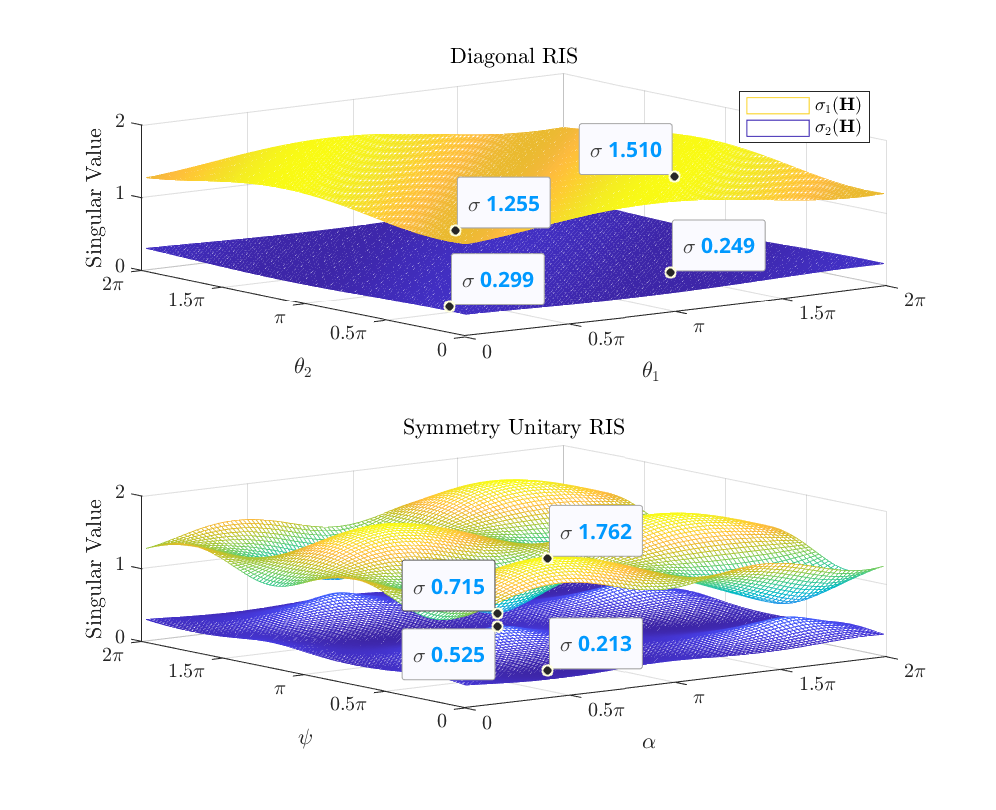
\includegraphics[width=\columnwidth]{assets/simulation/pc_singular_toy.eps}
			\caption{Channel singular value shaping by diagonal and symmetry unitary \gls{ris}. $(N^\mathrm{T}, N^\mathrm{S}, N^\mathrm{R}) = (2, 2, 2)$. Direct link is absent.}
			\label{sm:pc_singular_toy}
		\end{figure}
		Fig.~\ref{sm:pc_singular_toy} shows the channel singular values achieved by an exhaustive grid search over $(\theta_1, \theta_2)$ for diagonal \gls{ris} and $(\alpha, \psi)$ for symmetric unitary \gls{ris}.
		Interestingly, both singular values can be manipulated up to $9\%$ using diagonal \gls{ris} and $42\%$ using symmetric \gls{bd}-\gls{ris}, despite both architectures have the same number of angular parameters and scattering elements.
		A larger performance gap is expected when asymmetric \gls{bd}-\gls{ris} is available.
		This example shows \gls{bd}-\gls{ris} can provide a wider dynamic range of channel singular values.
		It emphasizes the importance of cooperative scattering and motivates further studies on channel shaping.
	\end{subsection}

	\begin{subsection}{Pareto Frontier Characterization}
		We then characterize the Pareto frontier of channel singular values by maximizing their weighted sum
		\begin{maxi!}
			{\scriptstyle{\mathbf{\Theta}}}{\sum_n \rho_n \sigma_n(\mathbf{H})}{\label{op:pc_singular}}{\label{ob:pc_singular}}
			\addConstraint{\mathbf{\Theta}_g^\mathsf{H} \mathbf{\Theta}_g=\mathbf{I}, \quad \forall g,}{}{}
		\end{maxi!}
		where $n \in \{1,\ldots,\min(N_\mathrm{T}, N_\mathrm{R})\}$ and $\rho_n$ is the weight of the $n$-th singular value that can be positive, zero, or negative.
		Varying $\{\rho_n\}$ allows us to explore the entire achievable singular value region.
		Problem~\eqref{op:pc_singular} thus generalizes all relevant metrics and provides a powerful channel shaping framework.
		For group $g$, the objective is smooth in $\mathbf{\Theta}_g$ and the feasible domain corresponds to the Stiefel manifold.
		% Those properties motivate us to propose a \gls{rcg} algorithm for smooth optimization problems of asymmetric \gls{bd}-\gls{ris} with arbitrary group size.
		% Those motivate us to propose a general \gls{rcg} algorithm for asymmetric \gls{bd}-\gls{ris} with arbitrary group size, which will be detailed in Section~\ref{sc:rcg}.
		Those properties motivate us to zoom out to general smooth optimization problems of asymmetric \gls{bd}-\gls{ris} with arbitrary group size.

		Inspired by \cite{Abrudan2008,Abrudan2009}, we propose a block-wise \gls{rcg} update along the geodesics on the Lie group of unitary matrices $\mathbb{U}^{L \times L}$.
		The gradient

		% It effectively solves general smooth asymmetric \gls{bd}-\gls{ris} problems with arbitrary group size.
		% The steps are summarized in Algorithm~\ref{ag:rcg}, where line \ref{ln:gradient_euclidean} computes the gradient in the Euclidean space, line \ref{ln:gradient_riemannian} translates it to the Riemannian manifold,
		% \footnote{The geodesics of the Stiefel manifold have compact expressions described by exponential map.}

% \footnote{The geodesics of the Stiefel manifold have compact expressions described by exponential map.}
		\setalgorithmcaptionfont{\small}
		\begin{algorithm}[!t]
			\small
			\caption{Block-wise \gls{rcg} update for asymmetric \gls{bd}-\gls{ris}}
			\label{ag:rcg}
			\begin{algorithmic}[1]
				\Require $f(\mathbf{\Theta})$, $G$
				\Ensure $\mathbf{\Theta}^\star$
				\State $r \gets 0$, $\mathbf{\Theta}^{(0)}$
				\Repeat
					\State $r \gets r+1$
					\For {$g \gets 1$ to $G$}
						\State $\nabla_{\mathrm{E},g}^{(r)} \gets {\partial f(\mathbf{\Theta}_g^{(r)})}/{\partial \mathbf{\Theta}_g^*}$\label{ln:gradient_euclidean}
						\State $\nabla_{\mathrm{R},g}^{(r)} \gets \nabla_{\mathrm{E},g}^{(r)} {\mathbf{\Theta}_g^{(r)}}^\mathsf{H} - \mathbf{\Theta}_g^{(r)} {\nabla_{\mathrm{E},g}^{(r)}}^\mathsf{H}$\label{ln:gradient_riemannian}
						\State $\gamma_g^{(r)} \gets {\mathrm{tr}\bigl((\nabla_{\mathrm{R},g}^{(r)} - \nabla_{\mathrm{R},g}^{(r-1)}) {\nabla_{\mathrm{R},g}^{(r)}}^\mathsf{H}\bigr)}/{\mathrm{tr}\bigl(\nabla_{\mathrm{R},g}^{(r-1)} {\nabla_{\mathrm{R},g}^{(r-1)}}^\mathsf{H}\bigr)}$\label{ln:parameter_polak_approx}
						\State $\mathbf{D}_g^{(r)} \gets \nabla_{\mathrm{R},g}^{(r)} + \gamma_g^{(r)} \mathbf{D}_g^{(r-1)}$\label{ln:direction_conjugate}
						\State $\mu_g^{(r)} \gets \arg\max_{\mu_g} f\bigl(\exp\bigl(\mu_g \mathbf{D}_g^{(r)}\bigr) \mathbf{\Theta}_g^{(r)}\bigr)$\label{ln:step_armijo}
						\State $\mathbf{\Theta}_g^{(r+1)} \gets \exp\bigl(\mu_g^{(r)} \mathbf{D}_g^{(r)}\bigr) \mathbf{\Theta}_g^{(r)}$\label{ln:update_geodesic}
					\EndFor
				\Until $\lvert R^{(r)} - R^{(r-1)} \rvert / R^{(r-1)} \le \epsilon$
			\end{algorithmic}
		\end{algorithm}


		% fun = @(Theta_g) rho' * svd(H_d + H_b(:, S) * Theta_g * H_f(S, :) + H_b(:, S_c) * Theta(S_c, S_c) * H_f(S_c, :));
		% G_e(S, S) = gradient_euclidean(H, H_f(S, :), H_b(:, S), rho);
		% G_r(S, S) = gradient_riemannian(Theta(S, S), G_e(S, S));
		% D(S, S) = direction_conjugate(G_r(S, S), struct('G_r', iter.G_r(S, S), 'D', iter.D(S, S), 'counter', iter.counter));
		% Theta(S, S) = step_armijo(fun, Theta(S, S), D(S, S));

		% we update $\mathbf{\Theta}$ by \gls{rcg} method along the geodesics.
		% \begin{remark}
		% 	A geodesic refers to the shortest path between two points in a Riemannian manifold.
		% 	% For unitary constraint \eqref{cs:pc_rate_unitary}, the
		% 	Unitary constraint \eqref{cs:pc_rate_unitary} translates to a Stiefel manifold where the geodesics have simple expressions described by the exponential map \cite{Abrudan2008}.
		% 	% Geodesics are the locally shortest paths in a Riemannian manifold.
		% 	% A Geodesics are the locally shortest paths in a Riemannian manifold.
		% 	% on Riemannian manifold are the shortest path between two points.
		% \end{remark}
		For general optimization problems with block unitary constraint, the adapted \gls{rcg} method at iteration $r$ for block $g$ is summarized below, where $f\bigl(\mathbf{\Theta}_g^{(r)}\bigr)$ is the objective function also evaluated over $\bigl\{ \{\mathbf{\Theta}_{g'}^{(r+1)}\}_{g'<g}, \{\mathbf{\Theta}_{g'}^{(r)}\}_{g'>g} \bigr\}$.
		\begin{enumerate}
			\item Compute the Euclidean gradient
			\begin{equation}
				{\nabla_g^\mathrm{E}}^{(r)} = \frac{\partial f\bigl(\mathbf{\Theta}_g^{(r)}\bigr)}{\partial \mathbf{\Theta}_g^*};
				\label{eq:rcg_gradient_euclidean}
			\end{equation}
			\item Translate to the Riemannian gradient
			\begin{equation}
				{\nabla_g^\mathrm{R}}^{(r)} = {\nabla_g^\mathrm{E}}^{(r)} {\mathbf{\Theta}_g^{(r)}}^\mathsf{H} - \mathbf{\Theta}_g^{(r)} {{\nabla_g^\mathrm{E}}^{(r)}}^\mathsf{H};
				\label{eq:rcg_gradient_riemannian}
			\end{equation}
			\item Determine the weight factor
			\begin{equation}
				\gamma_g^{(r)} = \frac{\mathrm{tr}\Bigl(\bigl({\nabla_g^\mathrm{R}}^{(r)} - {\nabla_g^\mathrm{R}}^{(r-1)}\bigr) {{\nabla_g^\mathrm{R}}^{(r)}}^\mathsf{H}\Bigr)}{\mathrm{tr}\Bigl({\nabla_g^\mathrm{R}}^{(r-1)} {{\nabla_g^\mathrm{R}}^{(r-1)}}^\mathsf{H}\Bigr)};
				\label{eq:rcg_weight}
			\end{equation}
			\item Compute the conjugate direction
			\begin{equation}
				\mathbf{D}_g^{(r)} = {\nabla_g^\mathrm{R}}^{(r)} + \gamma_g^{(r)} \mathbf{D}_g^{(r-1)};
				\label{eq:rcg_direction}
			\end{equation}
			\item Determine the Armijo step size\footnote{To double the step size, simply square the argument instead of recomputing the matrix exponential, i.e., $\exp(2 \mu_g \mathbf{D}_g) = \exp^2(\mu_g \mathbf{D}_g)$.}
			\begin{equation}
				\mu_g^{(r)} = \arg\max_{\mu_g} f\Bigl(\exp\bigl(\mu_g \mathbf{D}_g^{(r)}\bigr) \mathbf{\Theta}_g^{(r)}\Bigr);
				\label{eq:rcg_step}
			\end{equation}
			\item Perform rotational update along local geodesics
			\begin{equation}
				\mathbf{\Theta}_g^{(r+1)} = \exp\Bigl(\mu_g^{(r)} \mathbf{D}_g^{(r)}\Bigr) \mathbf{\Theta}_g^{(r)}.
				\label{eq:rcg_update}
			\end{equation}
		\end{enumerate}

		\begin{remark}
			The adapted \gls{rcg} method leverages the fact that block unitary matrices are closed under multiplication (but not necessarily under addition).
			Its advantage over universal manifold optimization \cite{Absil2009,Pan2022d} is trifold:
			\begin{itemize}
				\item No retraction is involved;
				\item Lower computational complexity per iteration \cite{Abrudan2008};
				\item Faster convergence thanks appropriate operational space.
			\end{itemize}
		\end{remark}

	\end{subsection}

	\begin{subsection}{Analytical Bounds}
		We then analyze the channel shaping \emph{capability} of \gls{bd}-\gls{ris} under specific setups.
		\begin{subsubsection}{Rank-Deficient Channel}
			\label{sc:pc_rank_deficient}
			In rank-deficient channels, \gls{bd}-\gls{ris} $\mathbf{\Theta}^\mathrm{B}$ cannot achieve a higher \gls{dof} than diagonal \gls{ris} $\mathbf{\Theta}^\mathrm{D}$.
			This is because $\mathrm{sv}(\mathbf{\Theta}^\mathrm{B}) = \mathrm{sv}(\mathbf{\Theta}^\mathrm{D}) = \boldsymbol{1}$ and
			\begin{equation}
				\begin{split}
					\mathrm{rank}(\mathbf{H})
					& \le \mathrm{rank}(\mathbf{H}^\mathrm{D}) + \mathrm{rank}(\mathbf{H}^\mathrm{B} \mathbf{\Theta} \mathbf{H}^\mathrm{F}) \\
					& \le \mathrm{rank}(\mathbf{H}^\mathrm{D}) + \min \bigl( \mathrm{rank}(\mathbf{H}^\mathrm{B}), \mathrm{rank}(\mathbf{\Theta}), \mathrm{rank}(\mathbf{H}^\mathrm{F}) \bigr).
				\end{split}
			\end{equation}
			% However, \gls{bd}-\gls{ris} can still guarantee a higher rate at finite \gls{snr}.
			Note \gls{bd}-\gls{ris} can still provide a higher indirect \gls{snr} as shown in Fig.~\ref{sm:pc_power_sx} and \ref{sm:pc_power_bond}.
		\end{subsubsection}


		\begin{subsubsection}{Rank-1 Indirect Channel}
			The indirect channel is rank-1 iff the forward or backward channel is rank-1.
			Let $\mathbf{H}^\mathrm{F} = \sigma^\mathrm{F} \mathbf{u}^\mathrm{F} {\mathbf{v}^\mathrm{F}}^\mathsf{H}$ without loss of generality.
			In this case, the channel Gram matrix can be written as Hermitian-plus-rank-1:
			\begin{equation}
				\mathbf{G} \triangleq \mathbf{H} \mathbf{H}^\mathsf{H} = \mathbf{Y} + \mathbf{z} \mathbf{z}^\mathsf{H},
			\end{equation}
			where $\mathbf{Y} \triangleq \mathbf{H}^\mathrm{D} (\mathbf{I} - \mathbf{v}^\mathrm{F} {\mathbf{v}^\mathrm{F}}^\mathsf{H}) \mathbf{H}^\mathrm{D} = \mathbf{T} \mathbf{T}^\mathsf{H}$ and $\mathbf{z} \triangleq \sigma^\mathrm{F} \mathbf{H}^\mathrm{B} \mathbf{\Theta} \mathbf{u}^\mathrm{F} + \mathbf{H}^\mathrm{D} \mathbf{v}^\mathrm{F}$.
			Regardless of \gls{ris} size and structure\footnote{A similar conclusion was made for diagonal \gls{ris} in \cite{Semmler2023}.}, its $n$-th ($n \ge 2$) eigenvalues are bounded by the Cauchy interlacing formula \cite{Golub2013}
			\begin{equation}
				\lambda_1(\mathbf{Y}) \ge {\color{blue}\lambda_2(\mathbf{G})} \ge \lambda_2(\mathbf{Y}) \ge \ldots \ge \lambda_{N-1}(\mathbf{Y}) \ge {\color{blue}\lambda_N(\mathbf{G})} \ge \lambda_N(\mathbf{Y}).
			\end{equation}
			The equivalent singular value inequality is
			\begin{equation}
				\sigma_1(\mathbf{T}) \ge {\color{blue}\sigma_2(\mathbf{H})} \ge \sigma_2(\mathbf{T}) \ge \ldots \ge \sigma_{N-1}(\mathbf{T}) \ge {\color{blue}\sigma_N(\mathbf{H})} \ge \sigma_N(\mathbf{T}).
				\label{iq:singular_value_interlacing}
			\end{equation}
			\eqref{iq:singular_value_interlacing} implies that, if the indirect channel is rank-1, then the \gls{ris} can at most enlarge the $n$-th ($n \ge 2$) channel singular value to the $(n-1)$-th singular value of $\mathbf{T}$.
			Note that the largest channel singular value is unbounded with a sufficiently large \gls{ris}.
		\end{subsubsection}

		\begin{subsubsection}{Fully-Connected \glsentryshort{ris} Without Direct Link}
			Denote the singular value decomposition of forward / backward channels as $\mathbf{H}^{\mathrm{B}/\mathrm{F}} = \mathbf{U}^{\mathrm{B}/\mathrm{F}} \mathbf{\Sigma}^{\mathrm{B}/\mathrm{F}} {\mathbf{V}^{\mathrm{B}/\mathrm{F}}}^\mathsf{H}$.
			The composite channel is
			\begin{equation}
				\mathbf{H} = \mathbf{H}^\mathrm{B} \mathbf{\Theta} \mathbf{H}^\mathrm{F} = \mathbf{U}^\mathrm{B} \mathbf{\Sigma}^\mathrm{B} \mathbf{X} \mathbf{\Sigma}^\mathrm{F} {\mathbf{V}^\mathrm{F}}^\mathsf{H},
			\end{equation}
			where $\mathbf{X} = {\mathbf{V}^\mathrm{B}}^\mathsf{H} \mathbf{\Theta} \mathbf{U}^\mathrm{F}$.
			% Since unitary matrices are closed under multiplication,
			\begin{proposition}
				In this case, the singular value bounds on $\mathbf{H}$ are equivalent to the singular value bounds on $\mathbf{BF}$, where $\mathbf{B}$ and $\mathbf{F}$ are arbitrary matrices with singular values $\mathbf{\Sigma}^\mathrm{B}$ and $\mathbf{\Sigma}^\mathrm{F}$.
				% The only singular value bounds applied here are those apply to the singular value bound of $\mathbf{F}\mathbf{B}$
			\end{proposition}
			\begin{proof}
				We first observe that singular value control problem can be solved w.r.t. unitary $\mathbf{X}$ and retrieved by $\mathbf{\Theta} = \mathbf{V}^\mathrm{B} \mathbf{X} {\mathbf{U}^\mathrm{F}}^\mathsf{H}$.
				Also, $\mathrm{sv}(\mathbf{U}^\mathrm{B} \mathbf{\Sigma}^\mathrm{B} \mathbf{X} \mathbf{\Sigma}^\mathrm{F} {\mathbf{V}^\mathrm{F}}^\mathsf{H}) = \mathrm{sv}(\bar{\mathbf{U}}^\mathrm{B} \mathbf{\Sigma}^\mathrm{B} \mathbf{\bar{V}}{{}^\mathrm{B}}^\mathsf{H} \bar{\mathbf{U}}^\mathrm{F} \mathbf{\Sigma}^\mathrm{F} \mathbf{\bar{V}}{{}^\mathrm{F}}^\mathsf{H}) = \mathrm{sv}(\mathbf{BF})$ where $\bar{\mathbf{U}}^{\mathrm{B}/\mathrm{F}}$ and $\bar{\mathbf{V}}^{\mathrm{B}/\mathrm{F}}$ are arbitrary unitary matrices.
			\end{proof}
			The problem now becomes, given $\mathbf{\Sigma}^\mathrm{B}$ and $\mathbf{\Sigma}^\mathrm{F}$, what can we say about the singular value of $\mathbf{BF}$.
			One comprehensive answer is Horn's inequality \cite{Bhatia2001}: for all admissible triples $(I, J, K)$,
			\begin{equation}
				\prod_{k \in {K}} \sigma_k(\mathbf{BF}) \leq \prod_{i \in {I}} \sigma_i(\mathbf{B}) \prod_{j \in {J}} \sigma_j(\mathbf{F}).
			\end{equation}
			It gives upper bound on the largest singular value and lower bound on the smallest singular value:
			\begin{align}
				\sigma_1(\mathbf{BF}) \le \sigma_1(\mathbf{B}) \sigma_1(\mathbf{F})\label{iq:singular_value_largest}\\
				\sigma_N(\mathbf{BF}) \geq \sigma_N(\mathbf{B}) \sigma_N(\mathbf{F})\label{iq:singular_value_smallest}.
			\end{align}
			Another useful result is introduced in \cite{Hogben2013}: for all $p>0$,
			\begin{equation}
				\sum_n \sigma_n^p(\mathbf{BF}) \leq \sum_n \sigma_n^p(\mathbf{B}) \sigma_n^p(\mathbf{F})\label{iq:singular_value_power_sum}.
			\end{equation}
			When $p=2$, it implies the channel energy is upper bounded by the sum of element-wise power product of the forward and backward channels, as illustrated in Fig.~\subref*{sm:pc_power_bond_nd}.
			Interestingly, \eqref{iq:singular_value_largest}--\eqref{iq:singular_value_power_sum} are simultaneously tight when $\mathbf{X} = \mathbf{I}$ and $\mathbf{\Theta} = \mathbf{V}^\mathrm{B} {\mathbf{U}^\mathrm{F}}^\mathsf{H}$.
			This solution was claimed in \cite{Bartoli2023} to achieve channel capacity, but it is not true at moderate \gls{snr}.
		\end{subsubsection}

		Finally, we characterize the \emph{Pareto frontier} of channel singular values via optimization approach.
		% \begin{maxi!}
		% 	{\scriptstyle{\mathbf{\Theta}}}{J_1 = \sum_n \rho_n \sigma_n(\mathbf{H})}{\label{op:pc_singular}}{\label{ob:pc_singular}}
		% 	\addConstraint{\mathbf{\Theta}_g^\mathsf{H} \mathbf{\Theta}_g=\mathbf{I}, \quad \forall g,}{}{}
		% \end{maxi!}


		% \begin{customopti!}
		% 	{\underset{\scriptstyle{\mathbf{\Theta}}}{max / min}}{}{J_1 = \sum_n \rho_n \sigma_n(\mathbf{H})}{\label{op:pc_singular}}{\label{ob:pc_singular}}
		% 	\addConstraint{\mathbf{\Theta}_g^\mathsf{H} \mathbf{\Theta}_g=\mathbf{I}, \quad \forall g,}{}{}
		% \end{customopti!}

		where $\rho_n$ is the weight of $n$-th singular value.
		The complex derivative of \eqref{ob:pc_singular} w.r.t. \gls{ris} block $g$ is
		\begin{equation}
			\frac{\partial J_1}{\partial \mathbf{\Theta}_g^*} = {\mathbf{H}_g^\mathrm{B}}^\mathsf{H} \mathbf{U} \mathrm{diag}(\boldsymbol{\rho}) \mathbf{V}^\mathsf{H} {\mathbf{H}_g^\mathrm{F}}^\mathsf{H},
			\label{eq:pc_singular_gradient_ris}
		\end{equation}
		where $\mathbf{U}$ and $\mathbf{V}$ are left and right singular matrix of $\mathbf{H}$.
		\eqref{op:pc_singular} can be solved by \gls{rcg} Algorithm~\ref{ag:pc_rate_ris} with \eqref{eq:pc_rate_gradient_ris} replaced by \eqref{eq:pc_singular_gradient_ris}.

		\begin{figure}[!t]
			\centering
			\resizebox{0.65\columnwidth}{!}{
				% This file was created by matlab2tikz.
%
%The latest updates can be retrieved from
%  http://www.mathworks.com/matlabcentral/fileexchange/22022-matlab2tikz-matlab2tikz
%where you can also make suggestions and rate matlab2tikz.
%
\definecolor{mycolor1}{rgb}{0.00000,0.44706,0.74118}%
\definecolor{mycolor2}{rgb}{0.85098,0.32549,0.09804}%
\definecolor{mycolor3}{rgb}{0.92941,0.69412,0.12549}%
\definecolor{mycolor4}{rgb}{0.49412,0.18431,0.55686}%
\definecolor{mycolor5}{rgb}{0.46667,0.67451,0.18824}%
\definecolor{mycolor6}{rgb}{0.30196,0.74510,0.93333}%
%
\begin{tikzpicture}

\begin{axis}[%
width=7.607cm,
height=6cm,
at={(0cm,0cm)},
scale only axis,
xmin=0.000780056016942828,
xmax=0.00151035544095343,
xlabel style={font=\color{white!15!black}},
xlabel={$\sigma_1$},
ymin=7.17325744537472e-06,
ymax=0.000678664297332486,
ylabel style={font=\color{white!15!black}},
ylabel={$\sigma_2$},
axis background/.style={fill=white},
xmajorgrids,
ymajorgrids,
legend style={at={(0.03,0.97)}, anchor=north west, legend cell align=left, align=left, draw=white!15!black},
every axis plot/.append style={line width=1.5pt}
]
\addplot[only marks, mark=triangle, mark options={}, mark size=2.3570pt, draw=black] table[row sep=crcr]{%
x	y\\
0.00114194570294393	0.000336225342793246\\
};
\addlegendentry{Direct}

\addplot [color=mycolor1, line width=2.0pt, mark=o, mark options={solid, mycolor1}]
  table[row sep=crcr]{%
0.00138310627521229	0.000541373661008476\\
0.00137650062985959	0.000547724709285543\\
0.00137179800217113	0.000551781207986263\\
0.0013667238895817	0.000555739545718357\\
0.00136112814892852	0.000559678324021497\\
0.00135487551639321	0.000563634744073936\\
0.00134775091714315	0.000567666443654481\\
0.00133936793517459	0.000571879549639873\\
0.00132911022650417	0.000576416739007263\\
0.00131599429418159	0.000581460348919756\\
0.0012967360881959	0.000587778982513483\\
0.00125291743622178	0.000599791200150401\\
0.00123119096742305	0.000604747849894878\\
0.00121706262307124	0.00060720968836112\\
0.00120312931454573	0.000608920098515012\\
0.00118319319377882	0.000610348651482186\\
0.00115877293143256	0.000610972503575572\\
0.00112102217893395	0.000610115716247662\\
0.00109378539134388	0.000608005728078314\\
0.00107029648027275	0.000605197393416344\\
0.00105547184744762	0.000602633418549789\\
0.00104213877218691	0.000599641355369312\\
0.00102799247140651	0.000595717570581489\\
0.00101243237813673	0.000590573859970719\\
0.00099765158108018	0.000584880420074443\\
0.000985474404824198	0.000579495304539842\\
0.000977054882138305	0.000575293715864339\\
0.000968493960895947	0.000570552195772108\\
0.000959448443947239	0.00056499444154939\\
0.000949762883346094	0.000558415417937255\\
0.000940898874894803	0.000551832918291931\\
0.000929694173301992	0.000542695545148083\\
0.000920850367351152	0.000534796819884117\\
0.000900829294210246	0.000514387538729727\\
0.000891072348660595	0.000503448155921158\\
0.000883349660057693	0.000494059504405429\\
0.000877381509040009	0.000486054603033194\\
0.000871889059839873	0.00047784724105625\\
0.000867274434238236	0.000470114648797319\\
0.000862879653329644	0.000461796103369074\\
0.000859004516703243	0.000453422359736673\\
0.000855302578009116	0.000444252984706068\\
0.000851893298834617	0.000434467965697125\\
0.000848592783927105	0.000423384711050787\\
0.000845670403449807	0.000411499031969129\\
0.000843321775663444	0.000399343270671556\\
0.000841605255954891	0.000387402178870989\\
0.000840395999717468	0.000375429510065964\\
0.000839351693789438	0.0003570937651608\\
0.000839191019418974	0.000327915448851247\\
0.000840689195489281	0.000281120846146895\\
0.000842130349022993	0.000265905448783712\\
0.00084409115613437	0.000252556420682459\\
0.000846538725629572	0.000240165771907757\\
0.000849204161049427	0.000229463788618431\\
0.000851884189549745	0.000220538386998371\\
0.000854854477792958	0.000212129929468686\\
0.000858078726410467	0.000204268009386366\\
0.000862057493895617	0.00019579533552623\\
0.000866183537849176	0.000187966603374027\\
0.000872685364376372	0.000176897203168152\\
0.000878035203258522	0.000168755365422576\\
0.000885115542229244	0.000159057883285553\\
0.000890259341893664	0.000152701169793039\\
0.000894445076657846	0.000148206832142025\\
0.000904528085778938	0.000137783784118971\\
0.000914043101821594	0.000128742525919212\\
0.000923627219793206	0.000120651609594527\\
0.000930618892641994	0.00011534268887723\\
0.000937546185180091	0.000110609972561044\\
0.000944208641424029	0.00010655384130683\\
0.000950889428800103	0.000102946892692312\\
0.00095798403046814	9.95699587129869e-05\\
0.000969025489849956	9.50708195368916e-05\\
0.00098780669720931	8.85150332311565e-05\\
0.00102925732960041	7.63083994196481e-05\\
0.00105007904621163	7.09154341096043e-05\\
0.0010679574569631	6.71669596953949e-05\\
0.00107823143506275	6.55813848899115e-05\\
0.00108999390516772	6.43936890140505e-05\\
0.0011146677521244	6.34278033979328e-05\\
0.00116760872987855	6.38388442047833e-05\\
0.0011989871467809	6.56978649469808e-05\\
0.0012271994780063	6.92824419993171e-05\\
0.00124195798799558	7.17728128000176e-05\\
0.00125049354883358	7.36854218185997e-05\\
0.00125997333623144	7.63255937293291e-05\\
0.00129023329588074	8.63046551108657e-05\\
0.0012984682901947	8.94672136844226e-05\\
0.00130588292099637	9.27593340770825e-05\\
0.0013168643843785	9.83004524971106e-05\\
0.00132528105595735	0.000103067181030408\\
0.0013353829965516	0.000109474010788843\\
0.00134373536077828	0.000115347073443698\\
0.00135143914505339	0.000121361141351383\\
0.0013593222011145	0.000128165492591833\\
0.00136779635126834	0.000136245347517388\\
0.00136780226909793	0.000136251265356634\\
0.00138007138749048	0.000149160589214526\\
0.00138717332522658	0.000157380671306964\\
0.00139409978877769	0.000166270534537689\\
0.00140124716417602	0.000176413211836964\\
0.00140749138662133	0.000186277315007801\\
0.0014135475852239	0.000196966385584272\\
0.00141870101441361	0.000207201634111093\\
0.00142393371257705	0.000219044065697338\\
0.00142986452445684	0.000234427164626466\\
0.00143451835718267	0.000248499910096157\\
0.00143914223977726	0.000265305517495102\\
0.00144318818589845	0.000283243464448841\\
0.00144577860424013	0.000298086525119162\\
0.00144740717914769	0.000311369832131257\\
0.00144911597987133	0.00033540414715251\\
0.001449740282944	0.000360440203198372\\
0.00144898155996544	0.000392979333980597\\
0.00144805747830175	0.00040597413311071\\
0.00144682624626129	0.000415968212527449\\
0.00144524441411516	0.000425106162134774\\
0.00144322075384459	0.000434098418144185\\
0.00144028900921996	0.00044465741764241\\
0.0014363258948624	0.000456641568539596\\
0.0014317521178514	0.000468504123638447\\
0.00142694134994165	0.000479367673175872\\
0.00142202909432219	0.000489130624624272\\
0.00141635599125354	0.000499130247987254\\
0.00140942153337546	0.000510080447601855\\
0.00140346432622276	0.000518567011414034\\
0.00139882031506131	0.00052452807904862\\
0.00139443228900829	0.000529615296352475\\
0.00138310627521229	0.000541373661008476\\
};
\addlegendentry{$L = 1$}

\addplot [color=mycolor2, dashed, line width=2.0pt, mark=+, mark options={solid, mycolor2}]
  table[row sep=crcr]{%
0.00142708402640716	0.000604787568359327\\
0.00142271915750979	0.000608943800481737\\
0.00141811975556122	0.000612911080424786\\
0.00141325985507629	0.00061670329126228\\
0.00140810262860234	0.000620334723659784\\
0.00140261050775027	0.000623811609422153\\
0.00139673468336242	0.000627139002579602\\
0.00139041687756152	0.0006303176150348\\
0.00138358351574295	0.000633344794552909\\
0.00137614656023266	0.000636211266192755\\
0.00136799984264635	0.000638899785050345\\
0.00135901564972722	0.0006413826822176\\
0.00134903632787048	0.000643619519976646\\
0.00133790074827829	0.000645546864487468\\
0.00132541778686717	0.000647080911786442\\
0.0013114194050922	0.000648107210139622\\
0.0012957234166404	0.000648484780759905\\
0.000965027022691634	0.000648174739122701\\
0.000953116391522089	0.000647327445150823\\
0.000942682856868463	0.000646044948041955\\
0.000933212575096715	0.000644405235164186\\
0.000924572712413129	0.000642468063807952\\
0.000916647548558176	0.00064027736999943\\
0.000909340403825754	0.000637865523868102\\
0.000902562843080782	0.000635252890955329\\
0.00089624816552161	0.000632455238085584\\
0.00089033540027291	0.00062948021989247\\
0.000885763283393741	0.000626906675131914\\
0.000880860459600062	0.000623860897261661\\
0.000876111014331454	0.000620597619806638\\
0.000871486123421155	0.000617088565984364\\
0.000867043758823932	0.000613371326973668\\
0.000864016574377116	0.000610632612917762\\
0.000846511269490986	0.000522019504583848\\
0.000838696416527526	0.000474071579566168\\
0.000821232684640372	0.000232862824041424\\
0.000820037997418569	0.000210159108579688\\
0.000819917252959101	0.000187368813972441\\
0.000820660633046176	0.000171196216937417\\
0.000821987746823761	0.000157301587104839\\
0.000823764747696633	0.000145107050371355\\
0.000825687984660003	0.00013531277127897\\
0.000827832813162708	0.00012661779842921\\
0.000830426121950891	0.000117971621347549\\
0.000832929298057577	0.00011094446318451\\
0.000835942984089802	0.000103648972286273\\
0.000838674103548881	9.78950379345763e-05\\
0.000841539217502674	9.25429928003555e-05\\
0.000844351201984642	8.78508012826726e-05\\
0.000847125900899661	8.36953862270355e-05\\
0.000849846919325928	8.00637518268895e-05\\
0.000852532289732515	7.69269119458458e-05\\
0.000866716878707244	6.26448433569685e-05\\
0.00087270371395697	5.70926243560763e-05\\
0.000877759373283318	5.30968239463015e-05\\
0.000882952600719378	4.95787883703482e-05\\
0.000888217052806595	4.63851988495259e-05\\
0.000893886726687168	4.33249700603755e-05\\
0.000900105634135452	4.03547417103093e-05\\
0.00090686018910192	3.75221836482069e-05\\
0.000914199831316421	3.48535258481474e-05\\
0.000922389286303664	3.23171217039454e-05\\
0.00093064196040592	3.01832536585429e-05\\
0.000940253992934137	2.81740909686967e-05\\
0.000952766968790558	2.62395802923065e-05\\
0.000963821000435015	2.51324235355461e-05\\
0.000974836617107741	2.45348800548086e-05\\
0.00116028175009671	2.40360113277235e-05\\
0.00132779736826404	2.50075272936491e-05\\
0.00133930850099718	2.64222260919868e-05\\
0.00134968102611387	2.82179466092547e-05\\
0.00135907593879845	3.0324228983548e-05\\
0.00136762408420579	3.26868521650145e-05\\
0.0013754503556155	3.52697505872883e-05\\
0.00138264420979487	3.80425983848555e-05\\
0.00138929404483273	4.09884323531799e-05\\
0.00139546935476089	4.40952617637862e-05\\
0.00140122813941479	4.7356208037743e-05\\
0.00140661912145658	5.0768771373459e-05\\
0.00141168559469095	5.43359583324757e-05\\
0.00141645528657518	5.80575457363142e-05\\
0.00142095335524875	6.1937048592521e-05\\
0.00142520794529952	6.59873276617985e-05\\
0.00142521279587381	6.59921843736945e-05\\
0.00142924075150828	7.02230594917907e-05\\
0.00143306521730864	7.4657105761573e-05\\
0.0014367014801233	7.93173741545556e-05\\
0.00144016674060654	8.42388733283363e-05\\
0.00144348050464032	8.94736363954968e-05\\
0.00144666254650657	9.5093695974115e-05\\
0.00144972023375186	0.000101172596553216\\
0.00145268165739489	0.000107859510420232\\
0.00145555680400201	0.000115322356145454\\
0.0014583565206516	0.000123811779409517\\
0.0014610636891567	0.000133616269215928\\
0.0014636191364663	0.000145026766688334\\
0.00146588288027385	0.000158114637133945\\
0.00146762077069576	0.000172666681034497\\
0.0014687735162738	0.000190221610719169\\
0.00146915290570309	0.000483033378294175\\
0.00146882549744291	0.00049668217313484\\
0.00146793216938846	0.000508860572040249\\
0.00146658198933905	0.000519842437077053\\
0.00146485605746963	0.000529809636327616\\
0.00146281875432854	0.000538895039264113\\
0.00146051555254218	0.000547226302947052\\
0.00145798265455466	0.000554899463086761\\
0.00145524614016565	0.000561998113218985\\
0.00145232130046503	0.000568599721328894\\
0.00144922613397254	0.000574751185224009\\
0.00144596069681674	0.000580517221036246\\
0.00144253311921193	0.000585930986247822\\
0.00143894001373822	0.000591033514755099\\
0.00143517245823788	0.000595861596864086\\
0.00143122397168896	0.00060043919514156\\
0.00142708402640716	0.000604787568359327\\
};
\addlegendentry{$L = 2$}

\addplot [color=mycolor3, dotted, line width=2.0pt, mark=square, mark options={solid, mycolor3}]
  table[row sep=crcr]{%
0.00147464710888256	0.000643844020909914\\
0.00147231745164227	0.0006460618476807\\
0.00146983457264343	0.000648203262268262\\
0.00146717996168842	0.000650274454033014\\
0.00146433100276465	0.000652280297805771\\
0.00146125832783688	0.000654225289330274\\
0.00145792844064094	0.000656110722793428\\
0.00145429832798864	0.00065793683405791\\
0.00145031802776613	0.000659699781367912\\
0.00144592536863341	0.000661392528945179\\
0.00144104285438955	0.000663003448195518\\
0.00143558082673444	0.000664512562293651\\
0.0014294244301872	0.00066589217051745\\
0.00142243728712495	0.000667101073222746\\
0.00141447558322257	0.000668078912291164\\
0.00140535669670137	0.000668746676408797\\
0.00139490598471284	0.00066899738594774\\
0.00088048299366601	0.000668812272853242\\
0.000873550086160286	0.000668303391407475\\
0.000867256013741648	0.000667529306482868\\
0.000861452598208385	0.000666523327803368\\
0.000856976108255466	0.000665528889989796\\
0.000854602424776079	0.000664873092304205\\
0.000852454662467834	0.000664164369298697\\
0.00085049610242013	0.000663409537094274\\
0.000848698492817159	0.000662613263704951\\
0.000847040644559746	0.000661779237579787\\
0.000845502540145749	0.000660908302262183\\
0.000844608057804923	0.00066035118469523\\
0.000843472305208182	0.000659584941346111\\
0.000842286176111254	0.000658708762277048\\
0.000841121225530027	0.000657763353867319\\
0.000840001593007474	0.000656764357352992\\
0.000812232940990677	0.000626421368891608\\
0.000809883204528856	0.000618139023411184\\
0.000807264852409728	0.000607997132639306\\
0.000805084914685545	0.000592271011124857\\
0.000803542457283137	0.000550510210063708\\
0.000800386432553601	0.000417493651337889\\
0.000794043883421996	9.0334877873103e-05\\
0.000793972127415645	7.97310291222311e-05\\
0.0007942822835895	7.29647431527983e-05\\
0.000794862696216749	6.69354646275064e-05\\
0.000795667251583902	6.14886128070505e-05\\
0.00079652877298028	5.71489429558201e-05\\
0.00079755718333706	5.30675850310195e-05\\
0.000798798205309549	4.90082192222722e-05\\
0.000799936890664325	4.58770732434572e-05\\
0.00080117195274252	4.29268210356955e-05\\
0.000802520126309781	4.01160573193132e-05\\
0.000803979158790408	3.74311019560697e-05\\
0.000805227182383533	3.53899029474618e-05\\
0.000806584577199513	3.34031959046927e-05\\
0.000807670131032197	3.19973445591675e-05\\
0.00081331540938068	2.62221957821652e-05\\
0.000817165720524356	2.24523957958149e-05\\
0.000819434354447684	2.05768423874612e-05\\
0.000821271576295598	1.92497161747541e-05\\
0.000823259499771728	1.78984635259949e-05\\
0.000825060981417118	1.6883945422112e-05\\
0.000827111641292875	1.58290226246866e-05\\
0.000828560736271671	1.51955454518116e-05\\
0.000830229513231851	1.45495899255563e-05\\
0.000832975712239036	1.36988542840672e-05\\
0.000835060490328013	1.31704737686185e-05\\
0.000837890660182347	1.25963384143438e-05\\
0.000840975354974674	1.21277262112687e-05\\
0.000844420019302498	1.17886649053315e-05\\
0.000847790010641279	1.15904178869432e-05\\
0.00110933061274061	1.15955039517421e-05\\
0.00147103492583293	3.24702028192906e-05\\
0.00147354964215683	3.51114094790464e-05\\
0.00147592405167717	3.78641349467274e-05\\
0.00147817057900536	4.07431110153949e-05\\
0.00148029780557032	4.37640717176944e-05\\
0.00148231370943686	4.69483493787478e-05\\
0.00148422139669122	5.03170001486611e-05\\
0.00148602660888332	5.39049327425515e-05\\
0.00148772566692037	5.77402153436902e-05\\
0.00148931790538428	6.1871078717496e-05\\
0.00149079397411919	6.63435805930189e-05\\
0.00149214303039024	7.12245890318055e-05\\
0.00149334518587021	7.65871721724621e-05\\
0.00149437237810609	8.25212370942591e-05\\
0.00149518484873857	8.91468940134306e-05\\
0.00149572327610295	9.67615422160606e-05\\
0.0014959282547223	0.000583245101104152\\
0.00149576610345023	0.000589994979930286\\
0.00149532780567967	0.000595969275190648\\
0.00149466881084009	0.000601329088459725\\
0.00149382669062799	0.000606192306186685\\
0.00149283121753642	0.000610630961324375\\
0.00149170477898718	0.00061470515751887\\
0.00149045883166532	0.000618479362467855\\
0.00148910670834217	0.000621986481325237\\
0.00148765268799133	0.000625268125788126\\
0.00148610115820591	0.000628351488022057\\
0.00148445304303643	0.000631261493494093\\
0.00148270736984734	0.000634018645406725\\
0.00148086018448727	0.00063664167753625\\
0.00147890637007859	0.000639145306451201\\
0.00147683835277814	0.000641542623529428\\
0.00147464710888256	0.000643844020909914\\
};
\addlegendentry{$L = 4$}

\addplot [color=mycolor4, dashdotted, line width=2.0pt, mark=x, mark options={solid, mycolor4}]
  table[row sep=crcr]{%
0.00149114449354831	0.000661719408573469\\
0.00148971067960646	0.000663084471805344\\
0.00148818556216129	0.000664399867367864\\
0.00148655769200873	0.000665670009421864\\
0.00148481563306035	0.000666896613322156\\
0.00148294214187752	0.000668082664997507\\
0.00148092001696473	0.00066922777217032\\
0.00147872695600218	0.000670331100359466\\
0.00147634094579288	0.000671388032657976\\
0.00147372924658086	0.000672394648300869\\
0.00147085456871825	0.000673343309532419\\
0.00146767332665402	0.000674222428028933\\
0.00146413355235245	0.000675015791139508\\
0.00146017046159136	0.000675701659880106\\
0.0014557044471	0.000676250382510514\\
0.00145063685434659	0.000676621609740527\\
0.00144485268664704	0.000676760345878413\\
0.00111301400180019	0.000676392038384927\\
0.000841152219364623	0.000676007418461906\\
0.000840272868504187	0.000675899360477419\\
0.000839480827291801	0.000675762252234721\\
0.000838761574203699	0.000675601000280695\\
0.000838104869203431	0.000675419481400017\\
0.000837500806265927	0.000675220111511114\\
0.000836942234565895	0.000675004799781134\\
0.000836423055478826	0.000674774790060942\\
0.000835937967071039	0.000674530717897867\\
0.000835483027536134	0.000674273078601584\\
0.000835054287444069	0.000674001648965441\\
0.000834805904759672	0.000673829680535123\\
0.000834469764017322	0.000673578357986569\\
0.000834115370008861	0.000673288477432602\\
0.000833765197425626	0.000672973818774901\\
0.000794202161770899	0.000633083920779501\\
0.000793867938887166	0.000632541141535194\\
0.00079352737805079	0.000631856453425249\\
0.000793215684427384	0.000631041262166604\\
0.000793043597945157	0.000630206880738918\\
0.000792704050881759	0.000628259602283743\\
0.000792307911954231	0.00062528787167064\\
0.000791784608941433	0.000620752979517279\\
0.000786800345896573	3.84109526067105e-05\\
0.000786787713010956	3.42060088493445e-05\\
0.000786924571333615	3.13935649070519e-05\\
0.00078717007865104	2.89232793341184e-05\\
0.000787520079937505	2.66688749586233e-05\\
0.000787916510930285	2.49131201439375e-05\\
0.000788799388854313	2.18376699125871e-05\\
0.000790046881874332	1.88432691446257e-05\\
0.000790399154239553	1.80334672104607e-05\\
0.000790820196185506	1.71953752799186e-05\\
0.000791146628146238	1.66175630518338e-05\\
0.000791457639352109	1.61246732201552e-05\\
0.000791727028731519	1.57562372493342e-05\\
0.000794257539857322	1.29799748099899e-05\\
0.000795051849493939	1.22713128229496e-05\\
0.000795667500001312	1.17786481253484e-05\\
0.000796528311814204	1.11867834471516e-05\\
0.000797122610698778	1.08305815243161e-05\\
0.000797943328709893	1.0389533823682e-05\\
0.000798867255380192	9.9586856766036e-06\\
0.000799827922406278	9.57250013972873e-06\\
0.000800582358379062	9.30661793928021e-06\\
0.000801961657636907	8.90710198185404e-06\\
0.000803654202381075	8.52307456881425e-06\\
0.000804720190372361	8.32335014562512e-06\\
0.000805944454034481	8.15421722137266e-06\\
0.000807438959740438	8.01364812865473e-06\\
0.00110691236266721	7.86238020497191e-06\\
0.00149209587705702	1.98354731775014e-05\\
0.00149326133695007	2.10597104740981e-05\\
0.00149437281036621	2.23483814132445e-05\\
0.00149543267414222	2.3706734580471e-05\\
0.00149644362712923	2.51425435318596e-05\\
0.00149740694884942	2.6664269731896e-05\\
0.00149832323291758	2.8282335923882e-05\\
0.0014991919255951	3.00089353941358e-05\\
0.00150001016415318	3.18559108232661e-05\\
0.00150077478298473	3.38394578118801e-05\\
0.00150148069959506	3.59781441913497e-05\\
0.00150211978023956	3.8290045830912e-05\\
0.00150268641050109	4.08206872229759e-05\\
0.00150325225166153	4.41067195679944e-05\\
0.0015037362264271	4.80419795567188e-05\\
0.00150405550011796	5.23929431961557e-05\\
0.00150417199080204	0.000624967288719598\\
0.00150407635710032	0.000628938208978892\\
0.00150381478075213	0.000632502731721301\\
0.0015034188029731	0.000635722568409952\\
0.00150290969093833	0.000638662390637057\\
0.00150230566130525	0.000641355719125861\\
0.00150161918951644	0.000643838766463172\\
0.00150085837523248	0.000646143525567912\\
0.00150002995989234	0.000648292192008007\\
0.00149913891538039	0.000650303036761557\\
0.00149818729365396	0.000652194097040846\\
0.00149717496611633	0.000653981472610825\\
0.00149610189528762	0.000655676255864267\\
0.00149496538964439	0.000657290040650924\\
0.00149376327370388	0.00065883035248372\\
0.0014924907498036	0.000660305436134498\\
0.00149114449354831	0.000661719408573469\\
};
\addlegendentry{$L = 8$}

\addplot [color=mycolor5, line width=2.0pt, mark=triangle, mark options={solid, mycolor5}]
  table[row sep=crcr]{%
0.00150176041534487	0.000670754051968293\\
0.00150100284662968	0.000671475312147767\\
0.00150019677331178	0.000672170603242325\\
0.00149933888307434	0.000672840033549226\\
0.00149842126910916	0.000673486187419973\\
0.00149743642438253	0.000674109662583373\\
0.00149637707807101	0.000674709564175822\\
0.00149522916267398	0.000675287109126198\\
0.0014939830697875	0.000675839125768933\\
0.00149261950977226	0.000676364682026978\\
0.00149112285912849	0.000676858565710381\\
0.00148946785148961	0.000677315916188379\\
0.00148762757152051	0.000677728392506179\\
0.00148556375154237	0.000678085554802152\\
0.00148323436196587	0.000678371664231412\\
0.00148058586954073	0.000678565610552767\\
0.00147753973706958	0.0006786386255264\\
0.000836495961475805	0.000678592074844945\\
0.000835644970060779	0.000678529701930123\\
0.0008348907667956	0.000678437063585258\\
0.000834219186066463	0.000678320835821318\\
0.000833617041102649	0.000678185868869332\\
0.00083307241045289	0.000678035364760581\\
0.000832576912463171	0.000677871860929263\\
0.000832123007955947	0.000677696934617009\\
0.000831704938005531	0.000677511756719791\\
0.00083131758958956	0.000677316890362505\\
0.00083095790479626	0.000677113223123577\\
0.000830621160101108	0.00067690005895894\\
0.000830481822557461	0.000676803966342334\\
0.00083027270374695	0.000676651238498501\\
0.00083003091899187	0.000676461136899916\\
0.000829778096236366	0.000676244927856991\\
0.000784727991534101	0.000631184204185072\\
0.000784535876603659	0.000630950309874341\\
0.000784295078900276	0.000630588973168354\\
0.000784063427970553	0.000630138864218799\\
0.000783564956495992	0.000628173344111054\\
0.00078164942806677	1.3835871559439e-05\\
0.000781866874311973	1.14466759595713e-05\\
0.000782088945679942	1.0450553335172e-05\\
0.000782165791034745	1.02010224383615e-05\\
0.00078265165035328	9.08029257163627e-06\\
0.000782708896678509	8.95536880617109e-06\\
0.000782783971031812	8.8204579218202e-06\\
0.000782882509187957	8.66803125170563e-06\\
0.000782993078442503	8.5608139981003e-06\\
0.000783642554672217	7.9536026157385e-06\\
0.000783771921288116	7.83593872442178e-06\\
0.000783875117385373	7.74603514354185e-06\\
0.000784017716494965	7.65535303867303e-06\\
0.000784146029860433	7.58245772077934e-06\\
0.00078428414065296	7.52149418335738e-06\\
0.000784673411971398	7.37693770922598e-06\\
0.000784871153087627	7.3101157329856e-06\\
0.000785291473686159	7.23652881656069e-06\\
0.000786537049874295	7.17325744537472e-06\\
0.00150503235768188	1.24928626919052e-05\\
0.00150549530249447	1.29824601614927e-05\\
0.00150584677431004	1.33910079911102e-05\\
0.00150620940821645	1.38558349774509e-05\\
0.00150654370266337	1.43306784992082e-05\\
0.00150685446206408	1.48216318666883e-05\\
0.00150713998562466	1.53258983046828e-05\\
0.00150740377605794	1.58501974812477e-05\\
0.00150764488334278	1.63944214739888e-05\\
0.00150786448513463	1.69640960977305e-05\\
0.00150806129710211	1.75603513009103e-05\\
0.00150823518492056	1.81892846262689e-05\\
0.00150838471418562	1.88568170624898e-05\\
0.00150850817659929	1.95740582208585e-05\\
0.00150860308332535	2.03698165444706e-05\\
0.00150877257325697	0.000650710270148995\\
0.00150871884149974	0.000652940822582109\\
0.00150857336767008	0.00065492399071795\\
0.00150835380516145	0.000656709919124592\\
0.00150807352891989	0.00065832837945251\\
0.00150774258923244	0.000659804014669009\\
0.00150736828223378	0.000661157894570665\\
0.00150695504553331	0.000662409683627243\\
0.00150650719419221	0.000663571300208811\\
0.00150602634194882	0.000664656485401296\\
0.00150551432526621	0.000665673913401069\\
0.00150497152714438	0.000666632213637762\\
0.00150439712837776	0.000667539319702475\\
0.00150379148037741	0.000668399270492002\\
0.00150315138420839	0.000669219474218465\\
0.00150247444276813	0.000670004158824613\\
0.00150176041534487	0.000670754051968293\\
};
\addlegendentry{$L = 16$}

\addplot [color=mycolor6, dashed, line width=2.0pt, mark=triangle, mark options={solid, rotate=180, mycolor6}]
  table[row sep=crcr]{%
0.00150451772041464	0.000672230748377712\\
0.00150388976633138	0.000672828585746527\\
0.00150322202264983	0.000673404534920682\\
0.00150251283385883	0.000673957870810169\\
0.00150175715265089	0.000674489945680385\\
0.00150094829672236	0.000675002008523016\\
0.00150007882063531	0.000675494385468285\\
0.00149914124120389	0.000675966095366154\\
0.00149812517380648	0.00067641620221792\\
0.00149701874264612	0.000676842641092354\\
0.00149580763322287	0.000677242291051333\\
0.00149447445781088	0.000677610684912327\\
0.00149299848328315	0.00067794148715916\\
0.0014913530623849	0.000678226272743749\\
0.00148950233847684	0.000678453655330355\\
0.00148740930755936	0.000678606950563539\\
0.00148501907679398	0.000678664297332486\\
0.000826537468795928	0.00067862104632937\\
0.000826416559018541	0.000678618766996447\\
0.000826386735923408	0.000678613669723356\\
0.000826365458606736	0.000678608167773506\\
0.000826352036142436	0.000678600565816895\\
0.000826339488451139	0.000678592621799651\\
0.00082632946243556	0.000678585617992278\\
0.000826318434799142	0.00067857715337961\\
0.000826307804929979	0.000678568138005092\\
0.000826297722087737	0.000678558695477075\\
0.000780158570996866	0.000631403902269862\\
0.000780125989532193	0.000624390377706646\\
0.000780056016942828	1.24522697650537e-05\\
0.000780154723074056	1.16232218687583e-05\\
0.000780602614165939	8.9723105343585e-06\\
0.000780637698083536	8.78250287518777e-06\\
0.000780657490575871	8.70825158373432e-06\\
0.000780696505964807	8.5716540389211e-06\\
0.000780715062014443	8.5282349431768e-06\\
0.000780786543960757	8.36649650352958e-06\\
0.00078080461300231	8.34680919973288e-06\\
0.000780831631416922	8.31954763790082e-06\\
0.000781959141292406	7.37072057948074e-06\\
0.000782191981327141	7.25089394744268e-06\\
0.000782344482940813	7.21246217707328e-06\\
0.000782784916914058	7.18152656899386e-06\\
0.000783122510976696	7.17928366958883e-06\\
0.0011415460560682	8.0419356072722e-06\\
0.00150315355760038	1.09554152080115e-05\\
0.0015043001597545	1.24833872765988e-05\\
0.0015064031387705	1.54371377748745e-05\\
0.00150700056125252	1.6329042693888e-05\\
0.00150836717874809	1.87001195776858e-05\\
0.00150880240373838	1.95529866567446e-05\\
0.00150904375427332	2.00587542327043e-05\\
0.00150939543825911	2.08942879958804e-05\\
0.00150959397034224	2.142360850482e-05\\
0.00150982884095011	2.21676735320339e-05\\
0.0015100279993965	2.29836001277622e-05\\
0.00151035544095343	0.000655608337400998\\
0.00151031145379601	0.000657430650033204\\
0.00151019170936605	0.000659062374446081\\
0.00151001024539879	0.000660537790298682\\
0.00150977800443558	0.000661878429939464\\
0.00150950300334766	0.000663104347450448\\
0.00150919121351512	0.000664231804437429\\
0.00150884669629331	0.000665275133450562\\
0.00150847291626886	0.000666244363913024\\
0.00150807201103746	0.000667148963394584\\
0.00150764477689351	0.000667997874750851\\
0.0015071918462329	0.000668797516522804\\
0.00150671308104189	0.000669553649087675\\
0.00150620862199329	0.000670270040792059\\
0.0015056739689034	0.000670955173265705\\
0.00150511217526256	0.000671606406105876\\
0.00150451772041464	0.000672230748377712\\
};
\addlegendentry{$L = 32$}

\end{axis}
\end{tikzpicture}%
			}
			\caption{Singular value Pareto frontier. $(N^\mathrm{T}, N^\mathrm{S}, N^\mathrm{R}) = (4, 64, 2)$, $(\Lambda^\mathrm{D}, \Lambda^\mathrm{F}, \Lambda^\mathrm{B}) = (0, -17.5, -17.5) \unit{dB}$.}
			\label{sm:pc_singular_pareto}
		\end{figure}

		\begin{figure}[!t]
			\centering
			\resizebox{0.65\columnwidth}{!}{
				% This file was created by matlab2tikz.
%
%The latest updates can be retrieved from
%  http://www.mathworks.com/matlabcentral/fileexchange/22022-matlab2tikz-matlab2tikz
%where you can also make suggestions and rate matlab2tikz.
%
\definecolor{mycolor1}{rgb}{0.58039,0.76863,0.96078}%
\definecolor{mycolor2}{rgb}{0.25882,0.37647,0.66667}%
\definecolor{mycolor3}{rgb}{0.94902,0.38039,0.38039}%
\definecolor{mycolor4}{rgb}{0.91765,0.03529,0.03529}%
\definecolor{mycolor5}{rgb}{0.46667,0.67451,0.18824}%
%
\begin{tikzpicture}

\begin{axis}[%
width=9.509cm,
height=7.5cm,
at={(0cm,0cm)},
scale only axis,
bar shift auto,
xmin=0,
xmax=5,
xtick={1,2,3,4},
xticklabels={{$\sigma_1$},{$\sigma_2$},{$\sigma_3$},{$\sigma_4$}},
ymin=0,
ymax=4.5,
ylabel style={font=\color{white!15!black}},
ylabel={Amplitude},
axis background/.style={fill=white},
xmajorgrids,
ymajorgrids,
legend style={legend cell align=left, align=left, draw=white!15!black},
legend columns=5,
transpose legend,
legend style={/tikz/column 2/.style={column sep=5pt}}
]
\addplot[ybar, bar width=0.123, fill=black, draw=black, area legend] table[row sep=crcr] {%
1	3.11578483462081\\
2	2.33621539044729\\
3	1.33501504737837\\
4	0.346232804852115\\
};
\addplot[forget plot, color=white!15!black] table[row sep=crcr] {%
0	0\\
5	0\\
};
\addlegendentry{Direct}

\addplot[ybar, bar width=0.123, fill=mycolor1, draw=black, area legend] table[row sep=crcr] {%
1	2.74905207049567\\
2	1.83843449000086\\
3	0.952844790933556\\
4	0.022527302733258\\
};
\addplot[forget plot, color=white!15!black] table[row sep=crcr] {%
0	0\\
5	0\\
};
\addlegendentry{Min, $L = 1$}

\addplot[ybar, bar width=0.123, fill=mycolor2, draw=black, area legend] table[row sep=crcr] {%
1	2.71936092735902\\
2	1.81605826060481\\
3	0.906339746943746\\
4	0.00914697809349159\\
};
\addplot[forget plot, color=white!15!black] table[row sep=crcr] {%
0	0\\
5	0\\
};
\addlegendentry{Min, $L = 32$}

\addplot[ybar, bar width=0.123, fill=mycolor3, draw=black, area legend] table[row sep=crcr] {%
1	3.8960081771894\\
2	2.67136418131802\\
3	1.64221742934803\\
4	0.603919247269453\\
};
\addplot[forget plot, color=white!15!black] table[row sep=crcr] {%
0	0\\
5	0\\
};
\addlegendentry{Max, $L = 1$}

\addplot[ybar, bar width=0.123, fill=mycolor4, draw=black, area legend] table[row sep=crcr] {%
1	4.03127940593837\\
2	2.67500105747776\\
3	1.67178857361767\\
4	0.628233917896107\\
};
\addplot[forget plot, color=white!15!black] table[row sep=crcr] {%
0	0\\
5	0\\
};
\addlegendentry{Max, $L = 32$}

\addplot [color=mycolor5, line width=2.0pt]
  table[row sep=crcr]{%
0	2.68074858002325\\
5	2.68074858002325\\
};
\addlegendentry{$\sigma_1(\mathbf{T})$}

\addplot [color=mycolor5, dashed, line width=2.0pt]
  table[row sep=crcr]{%
0	1.7029380545254\\
5	1.7029380545254\\
};
\addlegendentry{$\sigma_2(\mathbf{T})$}

\addplot [color=mycolor5, dotted, line width=2.0pt]
  table[row sep=crcr]{%
0	0.745179150575099\\
5	0.745179150575099\\
};
\addlegendentry{$\sigma_3(\mathbf{T})$}

\addplot [color=mycolor5, dashdotted, line width=2.0pt]
  table[row sep=crcr]{%
0	1.47492426026826e-08\\
5	1.47492426026826e-08\\
};
\addlegendentry{$\sigma_4(\mathbf{T})$}

\end{axis}

\begin{axis}[%
width=12.27cm,
height=9.202cm,
at={(-1.595cm,-1.012cm)},
scale only axis,
xmin=0,
xmax=1,
ymin=0,
ymax=1,
axis line style={draw=none},
ticks=none,
axis x line*=bottom,
axis y line*=left,
legend columns=5,
transpose legend,
legend style={/tikz/column 2/.style={column sep=5pt}}
]
\end{axis}
\end{tikzpicture}%
			}
			\caption{Singular value bounds for rank-1 indirect channel. $(N^\mathrm{T}, N^\mathrm{S}, N^\mathrm{R}) = (4, 32, 4)$, $(\Lambda^\mathrm{D}, \Lambda^\mathrm{F}, \Lambda^\mathrm{B}) = (0, -17.5, -17.5) \unit{dB}$.}
			\label{sm:pc_singular_bound}
		\end{figure}

		The Pareto frontier and evolving trend of channel singular values are shown in Fig.~\ref{sm:pc_singular_pareto} and \ref{sm:pc_singular_bound}.
		Clearly, \gls{bd}-\gls{ris} with a larger group size can redistribute the channel singular values to a wider range.
	\end{subsection}
	\begin{subsection}{Channel Power Maximization}
		Consider a \gls{bd}-\gls{ris} with $N^\mathrm{S}$ elements, which is divided into $G$ groups of equal $L$ elements.
		\begin{maxi!}
			{\scriptstyle{\mathbf{\Theta}}}{\left\lVert \mathbf{H}^\mathrm{D} + \sum_g\nolimits \mathbf{H}_g^\mathrm{B} \mathbf{\Theta}_g \mathbf{H}_g^\mathrm{F} \right\rVert _\mathrm{F}^2}{\label{op:pc_power}}{}
			\addConstraint{\mathbf{\Theta}_g^\mathsf{H} \mathbf{\Theta}_g=\mathbf{I}, \quad \forall g \in \mathcal{G} \triangleq \{1,\ldots,G\}.}{}{}
		\end{maxi!}
		For \emph{symmetric} BD-RIS, the problem has been solved in
		\begin{itemize}
			\item Matteo's paper \cite{Nerini2023}: SISO and equivalent\footnote{Single-stream MIMO with given precoder and combiner.};
			\item Ignacio's paper \cite{Santamaria2023}: SISO and directless MISO/SIMO.
		\end{itemize}

		\begin{remark}
			% The difficulty of \eqref{op:pc_power} is that the \gls{ris} needs to balance the (additive) direct-indirect eigenspace alignment and the (multiplicative) forward-backward eigenspace alignment.
			The difficulty of \eqref{op:pc_power} is that the \gls{ris} needs to balance the additive (direct-indirect) and multiplicative (forward-backward) eigenspace alignment.
			% align the direct and indirect eigenspaces while preserving the
			Interestingly, it has the same form as the \emph{weighted orthogonal Procrustes problem} \cite{Gower2004}:
			\begin{mini!}
				{\scriptstyle{\mathbf{\Theta}}}{\lVert \mathbf{C} - \mathbf{A \Theta B} \rVert _\mathrm{F}^2}{\label{op:weighted_orthogonal_procrustes}}{}
				\addConstraint{\mathbf{\Theta}^\mathsf{H} \mathbf{\Theta}=\mathbf{I}.}{}{}
			\end{mini!}
			There exists no trivial solution to \eqref{op:weighted_orthogonal_procrustes}.
			One lossy transformation, by moving $\mathbf{\Theta}$ to one side \cite{Bell2003}, formulates a standard orthogonal Procrustes problem:
			\begin{mini!}
				{\scriptstyle{\mathbf{\Theta}}}{\lVert \mathbf{A}^\dagger \mathbf{C} - \mathbf{\Theta B} \rVert _\mathrm{F}^2}{\label{op:standard_orthogonal_procrustes}}{}
				\addConstraint{\mathbf{\Theta}^\mathsf{H} \mathbf{\Theta}=\mathbf{I}.}{}{}
			\end{mini!}
			\eqref{op:standard_orthogonal_procrustes} has a global optimal solution $\mathbf{\Theta}^\star = \mathbf{U} \mathbf{V}^\mathsf{H}$, where $\mathbf{U}$ and $\mathbf{V}$ are left and right singular matrix of $\mathbf{\mathbf{A}^\dagger \mathbf{C} \mathbf{B}^\mathsf{H}}$ \cite{Golub2013}.
			This low-complexity solution will be compared with the one proposed later.
		\end{remark}

		Inspired by \cite{Nie2017}, we propose an iterative algorithm to solve \eqref{op:pc_power}.
		The idea is to successively approximate the quadratic objective with a sequence of affine functions and solve the resulting subproblems in closed form.

		\begin{proposition}
			Start from any $\mathbf{\Theta}^{(0)}$, the sequence
			\begin{equation}
				\mathbf{\Theta}_g^{(r+1)} = \mathbf{U}_g^{(r)} \mathbf{V}_g^{(r)}, \quad \forall g
			\end{equation}
			converges to a stationary point of \eqref{op:pc_power}, where $\mathbf{U}_g^{(r)}$ and $\mathbf{V}_g^{(r)}$ are left and right singular matrix of
			\begin{equation}
				\begin{split}
					\mathbf{M}_g^{(r)}
					& = {\mathbf{H}_g^\mathrm{B}}^\mathsf{H} \mathbf{H}^\mathrm{D} {\mathbf{H}_g^\mathrm{F}}^\mathsf{H} + \sum_{g' < g} {\mathbf{H}_{g'}^\mathrm{B}}^\mathsf{H} \mathbf{H}_{g'}^\mathrm{B} \mathbf{\Theta}_{g'}^{(r+1)} \mathbf{H}_{g'}^\mathrm{F} {\mathbf{H}_{g'}^\mathrm{F}}^\mathsf{H} \\
					& \quad + \sum_{g' \ge g} {\mathbf{H}_{g'}^\mathrm{B}}^\mathsf{H} \mathbf{H}_{g'}^\mathrm{B} \mathbf{\Theta}_{g'}^{(r)} \mathbf{H}_{g'}^\mathrm{F} {\mathbf{H}_{g'}^\mathrm{F}}^\mathsf{H}.
				\end{split}
			\end{equation}
		\end{proposition}

		\begin{proof}
			To be added.
		\end{proof}

		\begin{figure}[!t]
			\centering
			\resizebox{0.65\columnwidth}{!}{
				% This file was created by matlab2tikz.
%
%The latest updates can be retrieved from
%  http://www.mathworks.com/matlabcentral/fileexchange/22022-matlab2tikz-matlab2tikz
%where you can also make suggestions and rate matlab2tikz.
%
\definecolor{mycolor1}{rgb}{0.00000,0.44700,0.74100}%
\definecolor{mycolor2}{rgb}{0.00000,0.44706,0.74118}%
\definecolor{mycolor3}{rgb}{0.85000,0.32500,0.09800}%
\definecolor{mycolor4}{rgb}{0.85098,0.32549,0.09804}%
\definecolor{mycolor5}{rgb}{0.92900,0.69400,0.12500}%
\definecolor{mycolor6}{rgb}{0.92941,0.69412,0.12549}%
\definecolor{mycolor7}{rgb}{0.49400,0.18400,0.55600}%
\definecolor{mycolor8}{rgb}{0.49412,0.18431,0.55686}%
\definecolor{mycolor9}{rgb}{0.46600,0.67400,0.18800}%
\definecolor{mycolor10}{rgb}{0.46667,0.67451,0.18824}%
\definecolor{mycolor11}{rgb}{0.30100,0.74500,0.93300}%
\definecolor{mycolor12}{rgb}{0.50196,0.50196,0.50196}%
%
\begin{tikzpicture}

\begin{axis}[%
width=9.509cm,
height=7.5cm,
at={(0cm,0cm)},
scale only axis,
xmin=1,
xmax=9,
xtick={1,2,3,4,5,6,7,8,9},
xticklabels={{$2^0$},{$2^1$},{$2^2$},{$2^3$},{$2^4$},{$2^5$},{$2^6$},{$2^7$},{$2^8$}},
% xlabel style={font=\color{white!15!black}},
xlabel={RIS Group Size},
ymin=0,
ymax=0.000115972877397993,
% ylabel style={font=\color{white!15!black}},
ylabel={Channel Power [W]},
axis background/.style={fill=white},
xmajorgrids,
ymajorgrids,
legend style={at={(0.03,0.97)}, anchor=north west, legend cell align=left, align=left, draw=white!15!black}
]
\addplot[only marks, mark=o, mark options={}, mark size=1.5000pt, draw=mycolor2, forget plot] table[row sep=crcr]{%
x	y\\
5	7.97355699434511e-07\\
};
\addplot[only marks, mark=o, mark options={}, mark size=1.5000pt, draw=mycolor4, forget plot] table[row sep=crcr]{%
x	y\\
6	2.44467374534077e-06\\
};
\addplot[only marks, mark=o, mark options={}, mark size=1.5000pt, draw=mycolor6, forget plot] table[row sep=crcr]{%
x	y\\
7	8.20688590246789e-06\\
};
\addplot[only marks, mark=o, mark options={}, mark size=1.5000pt, draw=mycolor8, forget plot] table[row sep=crcr]{%
x	y\\
8	2.92944232352197e-05\\
};
\addplot[only marks, mark=o, mark options={}, mark size=1.5000pt, draw=mycolor10, forget plot] table[row sep=crcr]{%
x	y\\
9	0.000111116834986807\\
};
\addplot[only marks, mark=o, mark options={}, mark size=1.5000pt, draw=mycolor12] table[row sep=crcr]{%
x	y\\
nan	nan\\
};
\addlegendentry{Explicit}

\addplot [color=mycolor2, line width=2.0pt]
  table[row sep=crcr]{%
1	5.51363207462289e-07\\
2	6.17838345393838e-07\\
3	6.94081419821408e-07\\
4	7.63324397997057e-07\\
5	7.94677730055977e-07\\
};
\addlegendentry{$N_\mathrm{S} = 16$}

\addplot [color=mycolor4, dashed, line width=2.0pt]
  table[row sep=crcr]{%
1	1.30519166344131e-06\\
2	1.51964370152397e-06\\
3	1.79956076598358e-06\\
4	2.10847595748834e-06\\
5	2.3477592673609e-06\\
6	2.43406248970469e-06\\
};
\addlegendentry{$N_\mathrm{S} = 32$}

\addplot [color=mycolor6, dotted, line width=2.0pt]
  table[row sep=crcr]{%
1	3.16119975748769e-06\\
2	3.88133615484106e-06\\
3	4.87201167139358e-06\\
4	6.11096564201415e-06\\
5	7.28532076153866e-06\\
6	7.9551284625515e-06\\
7	8.16535091594136e-06\\
};
\addlegendentry{$N_\mathrm{S} = 64$}

\addplot [color=mycolor8, dashdotted, line width=2.0pt]
  table[row sep=crcr]{%
1	7.99146649497458e-06\\
2	1.02693781311302e-05\\
3	1.37563764650888e-05\\
4	1.84275764187614e-05\\
5	2.36208009984931e-05\\
6	2.71324017455215e-05\\
7	2.86565226414964e-05\\
8	2.91315486667727e-05\\
};
\addlegendentry{$N_\mathrm{S} = 128$}

\addplot [color=mycolor10, line width=2.0pt]
  table[row sep=crcr]{%
1	2.17362015080784e-05\\
2	2.95367070411585e-05\\
3	4.18294037335918e-05\\
4	5.98380359097175e-05\\
5	8.17678733318869e-05\\
6	9.81422641039276e-05\\
7	0.000106055811251013\\
8	0.000109356733903547\\
9	0.00011045035942666\\
};
\addlegendentry{$N_\mathrm{S} = 256$}

\end{axis}
\end{tikzpicture}%

			}
			\caption{Average channel power versus \gls{ris} elements $N^\mathrm{S}$ and group size $L$. $(N^\mathrm{T}, N^\mathrm{R}) = (8, 4)$, $(\Lambda^\mathrm{D}, \Lambda^\mathrm{F}, \Lambda^\mathrm{B}) = (65, 54, 46) \unit{dB}$.}
			\label{sm:pc_power_sx}
		\end{figure}

		\begin{figure}[!t]
			\centering
			\subfloat[Without Direct Link\label{sm:pc_power_bond_nd}]{
				\resizebox{0.48\columnwidth}{!}{
					% This file was created by matlab2tikz.
%
%The latest updates can be retrieved from
%  http://www.mathworks.com/matlabcentral/fileexchange/22022-matlab2tikz-matlab2tikz
%where you can also make suggestions and rate matlab2tikz.
%
\definecolor{mycolor1}{rgb}{0.46667,0.67451,0.18824}%
\definecolor{mycolor2}{rgb}{0.92941,0.50588,0.59608}%
%
\begin{tikzpicture}

\begin{axis}[%
width=7.607cm,
height=6cm,
at={(0cm,0cm)},
scale only axis,
bar shift auto,
xmin=0,
xmax=6,
xtick={1,2,3,4,5},
xticklabels={{1},{4},{16},{64},{256}},
xlabel style={font=\color{white!15!black}},
xlabel={RIS Group Size},
ymin=0,
ymax=3.5e-05,
ylabel style={font=\color{white!15!black}},
ylabel={Channel Power [W]},
axis background/.style={fill=white},
xmajorgrids,
ymajorgrids,
legend style={at={(0.03,0.97)}, anchor=north west, legend cell align=left, align=left, draw=white!15!black}
]
\addplot[ybar, bar width=0.8, fill=mycolor1, draw=black, area legend] table[row sep=crcr] {%
1	7.73646737868486e-07\\
2	1.29578759477113e-06\\
3	3.26134246923197e-06\\
4	8.76364407754596e-06\\
5	3.04057776451317e-05\\
};
\addplot[forget plot, color=white!15!black] table[row sep=crcr] {%
0	0\\
6	0\\
};
\addlegendentry{Composite}

\addplot [color=black, line width=2.0pt]
  table[row sep=crcr]{%
0	0\\
6	0\\
};
\addlegendentry{Direct}

\addplot [color=mycolor2, dashed, line width=2.0pt]
  table[row sep=crcr]{%
0	3.05527094461938e-05\\
6	3.05527094461938e-05\\
};
\addlegendentry{Cascaded}

\end{axis}
\end{tikzpicture}%
				}
			}
			\subfloat[With Direct Link\label{sm:pc_power_bond_hd}]{
				\resizebox{0.48\columnwidth}{!}{
					% This file was created by matlab2tikz.
%
%The latest updates can be retrieved from
%  http://www.mathworks.com/matlabcentral/fileexchange/22022-matlab2tikz-matlab2tikz
%where you can also make suggestions and rate matlab2tikz.
%
\definecolor{mycolor1}{rgb}{0.46667,0.67451,0.18824}%
\definecolor{mycolor2}{rgb}{0.92941,0.50588,0.59608}%
%
\begin{tikzpicture}

\begin{axis}[%
width=7.607cm,
height=6cm,
at={(0cm,0cm)},
scale only axis,
bar shift auto,
xmin=0,
xmax=6,
xtick={1,2,3,4,5},
xticklabels={{1},{4},{16},{64},{256}},
xlabel style={font=\color{white!15!black}},
xlabel={RIS Group Size},
ymin=0,
ymax=7e-05,
ylabel style={font=\color{white!15!black}},
ylabel={Channel Power [W]},
axis background/.style={fill=white},
xmajorgrids,
ymajorgrids,
legend style={at={(0.03,0.97)}, anchor=north west, legend cell align=left, align=left, draw=white!15!black}
]
\addplot[ybar, bar width=0.8, fill=mycolor1, draw=black, area legend] table[row sep=crcr] {%
1	2.83336295997331e-05\\
2	4.76924466169225e-05\\
3	6.08890936283682e-05\\
4	6.46004645413477e-05\\
5	6.64188484186803e-05\\
};
\addplot[forget plot, color=white!15!black] table[row sep=crcr] {%
0	0\\
6	0\\
};
\addlegendentry{Composite}

\addplot [color=black, line width=2.0pt]
  table[row sep=crcr]{%
-0.2	9.51300474293446e-06\\
6.2	9.51300474293446e-06\\
};
\addlegendentry{Direct}

\addplot [color=mycolor2, line width=2.0pt]
  table[row sep=crcr]{%
-0.2	3.07152044114707e-05\\
6.2	3.07152044114707e-05\\
};
\addlegendentry{Cascaded}

\end{axis}
\end{tikzpicture}%
				}
			}
			\caption{Average channel power versus \gls{ris} group size $L$. $(N^\mathrm{T}, N^\mathrm{S}, N^\mathrm{R}) = (8, 256, 4)$, $(\Lambda^\mathrm{D}, \Lambda^\mathrm{F}, \Lambda^\mathrm{B}) = (65, 54, 46) \unit{dB}$.}
			\label{sm:pc_power_bond}
		\end{figure}
		% Fig.~\ref{sm:pc_power_sx} shows that, apart from numerous reflecting elements, a sufficiently large group size can help
		% Fig.~\ref{sm:pc_power_sx} shows that increasing the group size can improve the channel power especially for a large \gls{ris}.
		Fig.~\ref{sm:pc_power_sx} shows that, apart from adding reflecting elements $N^\mathrm{S}$, increasing the group size $L$ also improves the channel power.
		% The behavior is more obvious for a large \gls{ris}.
		This behavior is more pronounced for a large \gls{ris}.
		For example, the gain of pairwise connection is \qty{2.8}{\percent} for $N^\mathrm{S} = 16$ and \qty{28}{\percent} for $N^\mathrm{S} = 256$.
		% \gls{bd}-\gls{ris} provides a higher channel power than conventional \gls{ris}.
		% As $L$ increases from 1 to 2,
		It implies that the channel shaping capability of \gls{bd}-\gls{ris} scales with group size $L$.

		Fig.~\ref{sm:pc_power_bond_hd} and \ref{sm:pc_power_bond_nd} compare the average channel power without and with direct link.
		% where the cascaded channel power available to passive \gls{ris} is $\lVert \mathbf{H}^\mathrm{B} \rVert _\mathrm{F}^2 \lVert \mathbf{H}^\mathrm{F} \rVert _\mathrm{F}^2$.
		% where the cascaded channel power available to passive \gls{ris} is $\lVert \mathbf{H}^\mathrm{B} \rVert _\mathrm{F}^2 \lVert \mathbf{H}^\mathrm{F} \rVert _\mathrm{F}^2$.
		% ``Cascaded'' means the maximum power of the cascaded channel, i.e., $\lVert \mathbf{H}^\mathrm{B} \rVert _\mathrm{F}^2 \lVert \mathbf{H}^\mathrm{F} \rVert _\mathrm{F}^2$.
		% maximum power of the cascaded channel, i.e., $\lVert \mathbf{H}^\mathrm{B} \rVert _\mathrm{F}^2 \lVert \mathbf{H}^\mathrm{F} \rVert _\mathrm{F}^2$.
		% ? ``Cascaded'' means the \emph{power product} of the forward and backward channels.
		% ``Cascaded'' means the sum of element-wise product of first $N = \min(N^\mathrm{T}, N^\mathrm{S}, N^\mathrm{R})$ eigenvalues of the forward and backward channels.
		``Cascaded'' means the sum of element-wise product of first $N = \min(N^\mathrm{T}, N^\mathrm{S}, N^\mathrm{R})$ eigenvalues (i.e., element-wise power product) of the forward and backward channels.
		We observe that diagonal \gls{ris} wastes substantial cascaded power and struggles to align the direct-indirect eigenspace.
		When the direct link is absent, only \qty{2.6}{\percent} of available power is utilized by diagonal \gls{ris} while \qty{100}{\percent} power is recycled by fully-connected \gls{ris}.
		When the direct link is present, the proposed \gls{bd}-\gls{ris} design can balance the direct-indirect and forward-backward eigenspace alignment for an optimal channel boost.
		It is worth noting that, when $L$ is sufficiently large, the composite channel power surpasses the power sum of direct and cascaded channels, thanks to the constructive \emph{amplitude superposition} of direct and cascaded channels.
		This again emphasizes the advantage of in-group connection of \gls{bd}-\gls{ris}.
		% This is because the direct and indirect channels superpose
		% the proposed \gls{bd}-\gls{ris} design can also be applied to conventional \gls{ris} to improve the channel power.
		% When the direct link is present, a small $L$ cannot align the direct-indirect eigenspace.

		% neither effectively utilizes the cascaded channel power, nor effectively align the direct-indirect eigenspace.
		% We observe that conventional \gls{ris} neither effectively utilizes the cascaded channel power, nor effectively align the direct-indirect eigenspace.
		% For conventional \gls{ris},
		% align the direct-indirect eigenspace.
		% When the direct link is present, a small $L$ can neither align the direct-indirect eigenspace nor the forward-backward eigenspace.
		% For a relatively large $N^\mathrm{S}$, conventional \gls{ris} cannot
		% neither the direct-indirect nor the forward-backward eigenspace can be effectively aligned with a small $L$.

		% When the direct link is present, a small $L$ can neither preserve the
		% neither align the direct-indirect eigenspace nor the forward-backward eigenspace.

		% When the direct link is absent, a large $L$ can align the forward-backward eigenspace but cannot preserve the forward-backward power balance.
	\end{subsection}

	\begin{subsection}{Rate Maximization}
		The problem is formulated w.r.t. precoder (instead of transmit covariance matrix) for reference:
		\begin{maxi!}
			{\scriptstyle{\mathbf{W},\mathbf{\Theta}}}{R = \log \det \biggl(\mathbf{I} + \frac{\mathbf{W}^\mathsf{H}\mathbf{H}^\mathsf{H}\mathbf{H}\mathbf{W}}{\eta}\biggr)}{\label{op:pc_rate}}{\label{ob:pc_rate}}
			\addConstraint{\lVert \mathbf{W} \rVert _\mathrm{F}^2 \le P}{}{}
			\addConstraint{\mathbf{\Theta}_g^\mathsf{H} \mathbf{\Theta}_g=\mathbf{I}, \quad \forall g.}{}{\label{cs:pc_rate_unitary}}
		\end{maxi!}

		\eqref{op:pc_rate} is jointly non-convex and solved by \gls{ao}.
		For a given $\mathbf{\Theta}$, the optimal precoder is given by
		\begin{equation}
			\mathbf{W}^\star = \mathbf{V} {\mathbf{S}^\star}^{1/2},
		\end{equation}
		where $\mathbf{V}$ is right singular matrix of $\mathbf{H}$ and $\mathbf{S}^\star$ is a diagonal matrix of the water-filling power allocation.
		For a given $\mathbf{W}$,
		The complex derivative of \eqref{ob:pc_rate} w.r.t. \gls{ris} block $g$ is
		\begin{equation}
			\frac{\partial R}{\partial \mathbf{\Theta}_g^*} = \frac{1}{\eta} {\mathbf{H}_g^\mathrm{B}}^\mathsf{H} \mathbf{HW} \biggl(\mathbf{I} + \frac{\mathbf{W}^\mathsf{H}\mathbf{H}^\mathsf{H}\mathbf{H}\mathbf{W}}{\eta}\biggr)^{-1} \mathbf{W}^\mathsf{H} {\mathbf{H}_g^\mathrm{F}}^\mathsf{H}.
			\label{eq:pc_rate_gradient_ris}
		\end{equation}
		Algorithm~\ref{ag:pc_rate_ris} summarizes the adapted \gls{rcg} method for the \gls{ris} rate maximization subproblem.

		\setalgorithmcaptionfont{\small}
		\begin{algorithm}[!t]
			\small
			\caption{\gls{rcg} Method for \gls{ris} \gls{mimo}-\gls{pc} Rate Maximization}
			\label{ag:pc_rate_ris}
			\begin{algorithmic}[1]
				\Require $\mathbf{H}^\mathrm{D}$, $\mathbf{H}^\mathrm{F}$, $\mathbf{H}^\mathrm{B}$, $\mathbf{W}$, $L$, $\eta$
				\Ensure $\mathbf{\Theta}^\star$
				\State $r \gets 0$, $\mathbf{\Theta}^{(0)}$
				\Repeat
					\State $r \gets r+1$
					\For {$g \gets 1$ to $G$}
						\State $\mathbf{\Theta}_g^{(r)} \gets$ \eqref{eq:pc_rate_gradient_ris}, \eqref{eq:rcg_gradient_riemannian}--\eqref{eq:rcg_update}
					\EndFor
				\Until $\lvert R^{(r)} - R^{(r-1)} \rvert / R^{(r-1)} \le \epsilon$
			\end{algorithmic}
		\end{algorithm}

		\begin{figure}[!t]
			\centering
			\subfloat[\gls{ris} Elements, $N^\mathrm{T} = 8$\label{sm:pc_rate_sx}]{
				\resizebox{0.48\columnwidth}{!}{
					% This file was created by matlab2tikz.
%
%The latest updates can be retrieved from
%  http://www.mathworks.com/matlabcentral/fileexchange/22022-matlab2tikz-matlab2tikz
%where you can also make suggestions and rate matlab2tikz.
%
\definecolor{mycolor1}{rgb}{0.00000,0.44706,0.74118}%
\definecolor{mycolor2}{rgb}{0.85098,0.32549,0.09804}%
%
\begin{tikzpicture}

\begin{axis}[%
width=9.509cm,
height=7.5cm,
at={(0cm,0cm)},
scale only axis,
xmin=-10,
xmax=30,
% xlabel style={font=\color{white!15!black}},
xlabel={Direct SNR [dB]},
ymin=0,
ymax=60,
% ylabel style={font=\color{white!15!black}},
ylabel={Achievable Rate [bit/s/Hz]},
axis background/.style={fill=white},
xmajorgrids,
ymajorgrids,
legend style={at={(0.03,0.97)}, anchor=north west, legend cell align=left, align=left, draw=white!15!black}
]
\addplot [color=black, line width=2.0pt]
  table[row sep=crcr]{%
-10	1.56187406999523\\
0	6.23295532679222\\
10	16.2843611075538\\
20	29.0985448133738\\
30	42.3364873073222\\
};
\addlegendentry{$N^\mathrm{S} = 0$}

\addplot [color=mycolor1, line width=2.0pt, mark=o, mark options={solid, mycolor1}]
  table[row sep=crcr]{%
-10	1.79403005594775\\
0	6.8098358611215\\
10	17.3483481001009\\
20	30.2902015018505\\
30	43.5423539886115\\
};
\addlegendentry{$(N^\mathrm{S}, L) = (32, 1)$}

\addplot [color=mycolor1, dashed, line width=2.0pt, mark=o, mark options={solid, mycolor1}]
  table[row sep=crcr]{%
-10	1.89438152702937\\
0	7.29195763868557\\
10	18.263799283564\\
20	31.2683950185117\\
30	44.5273711067635\\
};
\addlegendentry{$(N^\mathrm{S}, L) = (32, 4)$}

\addplot [color=mycolor1, dotted, line width=2.0pt, mark=o, mark options={solid, mycolor1}]
  table[row sep=crcr]{%
-10	1.92343952356708\\
0	7.54110875822535\\
10	18.7215302432174\\
20	31.7486185374994\\
30	45.0095773639065\\
};
\addlegendentry{$(N^\mathrm{S}, L) = (32, 32)$}

\addplot [color=mycolor2, line width=2.0pt, mark=+, mark options={solid, mycolor2}]
  table[row sep=crcr]{%
-10	3.23524840027798\\
0	10.4732909366393\\
10	22.9609501734511\\
20	36.1430515763993\\
30	49.4201986024039\\
};
\addlegendentry{$(N^\mathrm{S}, L) = (256, 1)$}

\addplot [color=mycolor2, dashed, line width=2.0pt, mark=+, mark options={solid, mycolor2}]
  table[row sep=crcr]{%
-10	3.98868943719332\\
0	12.8610741472271\\
10	26.1986080126589\\
20	39.4301968233646\\
30	52.7116073420547\\
};
\addlegendentry{$(N^\mathrm{S}, L) = (256, 4)$}

\addplot [color=mycolor2, dotted, line width=2.0pt, mark=+, mark options={solid, mycolor2}]
  table[row sep=crcr]{%
-10	4.95164015944269\\
0	15.3108768293702\\
10	28.201929438041\\
20	41.4467820962475\\
30	54.7294483831401\\
};
\addlegendentry{$(N^\mathrm{S}, L) = (256, 256)$}

\end{axis}

\begin{axis}[%
width=12.27cm,
height=9.202cm,
at={(-1.595cm,-1.012cm)},
scale only axis,
xmin=0,
xmax=1,
ymin=0,
ymax=1,
axis line style={draw=none},
ticks=none,
axis x line*=bottom,
axis y line*=left
]
\end{axis}
\end{tikzpicture}%

				}
			}
			\subfloat[Transmit Antenna, $N^\mathrm{S} = 256$\label{sm:pc_rate_tx}]{
				\resizebox{0.48\columnwidth}{!}{
					% This file was created by matlab2tikz.
%
%The latest updates can be retrieved from
%  http://www.mathworks.com/matlabcentral/fileexchange/22022-matlab2tikz-matlab2tikz
%where you can also make suggestions and rate matlab2tikz.
%
\definecolor{mycolor1}{rgb}{0.00000,0.44706,0.74118}%
\definecolor{mycolor2}{rgb}{0.85098,0.32549,0.09804}%
\definecolor{mycolor3}{rgb}{0.92941,0.69412,0.12549}%
%
\begin{tikzpicture}

\begin{axis}[%
width=9.509cm,
height=7.5cm,
at={(0cm,0cm)},
scale only axis,
xmin=-10,
xmax=30,
% xlabel style={font=\color{white!15!black}},
xlabel={Direct SNR [dB]},
ymin=0,
ymax=60,
% ylabel style={font=\color{white!15!black}},
ylabel={Achievable Rate [bit/s/Hz]},
axis background/.style={fill=white},
xmajorgrids,
ymajorgrids,
legend style={at={(0.03,0.97)}, anchor=north west, legend cell align=left, align=left, draw=white!15!black}
]
\addplot [color=mycolor1, line width=2.0pt, mark=o, mark options={solid, mycolor1}]
  table[row sep=crcr]{%
-10	1.82485438191362\\
0	4.7222906563119\\
10	7.99393509732638\\
20	11.3107371667968\\
30	14.6321519880831\\
};
\addlegendentry{$(N^\mathrm{T}, L) = (1, 1)$}

\addplot [color=mycolor1, dashed, line width=2.0pt, mark=o, mark options={solid, mycolor1}]
  table[row sep=crcr]{%
-10	2.24659926648999\\
0	5.26330445507328\\
10	8.55078517680736\\
20	11.8692222057207\\
30	15.1908007320325\\
};
\addlegendentry{$(N^\mathrm{T}, L) = (1, 256)$}

\addplot [color=mycolor2, line width=2.0pt, mark=+, mark options={solid, mycolor2}]
  table[row sep=crcr]{%
-10	2.49039510987196\\
0	8.06192104582032\\
10	17.6588170852107\\
20	32.7099587384036\\
30	45.9789160838128\\
};
\addlegendentry{$(N^\mathrm{T}, L) = (4, 1)$}

\addplot [color=mycolor2, dashed, line width=2.0pt, mark=+, mark options={solid, mycolor2}]
  table[row sep=crcr]{%
-10	3.77849180447307\\
0	13.3359194935281\\
10	26.0483499099173\\
20	39.2753832167713\\
30	52.5569826592083\\
};
\addlegendentry{$(N^\mathrm{T}, L) = (4, 256)$}

\addplot [color=mycolor3, line width=2.0pt, mark=square, mark options={solid, mycolor3}]
  table[row sep=crcr]{%
-10	3.8179809156775\\
0	12.9043718464691\\
10	25.5833268533688\\
20	38.8067308900334\\
30	52.0881220415066\\
};
\addlegendentry{$(N^\mathrm{T}, L) = (16, 1)$}

\addplot [color=mycolor3, dashed, line width=2.0pt, mark=square, mark options={solid, mycolor3}]
  table[row sep=crcr]{%
-10	5.83961863479039\\
0	16.7543020939844\\
10	29.7401886345762\\
20	42.9967723667009\\
30	56.2807797979848\\
};
\addlegendentry{$(N^\mathrm{T}, L) = (16, 256)$}

\end{axis}

\begin{axis}[%
width=12.27cm,
height=9.202cm,
at={(-1.595cm,-1.012cm)},
scale only axis,
xmin=0,
xmax=1,
ymin=0,
ymax=1,
axis line style={draw=none},
ticks=none,
axis x line*=bottom,
axis y line*=left
]
\end{axis}
\end{tikzpicture}%

				}
			}
			\caption{Average achievable rate versus group size $L$. $N^\mathrm{R} = 4$, $(\Lambda^\mathrm{D}, \Lambda^\mathrm{F}, \Lambda^\mathrm{B}) = (65, 54, 46) \unit{dB}$.}
			\label{sm:pc_rate}
		\end{figure}

		Fig.~\ref{sm:pc_rate_sx} illustrates how \gls{ris} configuration influences the \gls{mimo} \gls{pc} achievable rate.
		To ensure a \qty{20}{bit/s/Hz} transmission, an \gls{snr} of \qty{13.5}{\dB} is required for a 8T4R system.
		This value decreases to \qty{12.5}{\dB} (resp. \qty{8}{\dB}) when 32- (resp. 256-) element diagonal \gls{ris} is present.
		If tetrads can be formed in \gls{bd}-\gls{ris}, the \gls{snr} can be reduced by another \qty{20}{\percent} (resp. \qty{44}{\percent}).
		Further increase in $L$ yields a marginal gain and incurs $\mathcal{O}(L^2)$ connections.
		We thus conclude dyadic or tetradic \gls{bd}-\gls{ris} usually strike a good balance between performance and complexity.
	\end{subsection}

\end{section}

\begin{section}{\glsentryshort{mimo}-\glsentryshort{ic}}
	\begin{subsection}{Leakage Interference Minimization}
		\begin{mini!}
			{\scriptstyle{\mathbf{\Theta}, \{\mathbf{G}_k\}, \{\mathbf{W}_k\}}}{\mathop{\sum\sum}_{j \neq k} \left\lVert \mathbf{G}_k (\mathbf{H}_{kj}^\mathrm{D} + \mathbf{H}_k^\mathrm{B} \mathbf{\Theta} \mathbf{H}_j^\mathrm{F}) \mathbf{W}_j \right\rVert _{\mathrm{F}}^2}{}{}
			\addConstraint{\mathbf{\Theta}_g^\mathsf{H} \mathbf{\Theta}_g=\mathbf{I}, \quad \forall g}{}{}
			\addConstraint{\mathbf{G}_k \mathbf{G}_k^\mathsf{H}=\mathbf{I}, \quad \mathbf{W}_k^\mathsf{H} \mathbf{W}_k=\mathbf{I}, \quad \forall k.}{}{}
		\end{mini!}
		The non-convex problem can be solved by \gls{bcd} method.
		For a given $\mathbf{\Theta}$, it reduces to conventional linear beamforming problem, for which an iterative algorithm alternating between the original and reciprocal networks is proposed in \cite{Gomadam2011,Clerckx2013}.
		At iteration $r$, the combiner at receiver $k$ is updated as
		\begin{equation}
			\mathbf{G}_k^{(r)} = {\mathbf{U}_{k,N}^{(r-1)}}^\mathsf{H},
		\end{equation}
		where $\mathbf{U}_{k,N}^{(r-1)}$ is the eigenvectors corresponding to $N$ smallest eigenvalues of interference covariance matrix $\mathbf{Q}_k^{(r-1)} = \sum_{j \ne k} \mathbf{H}_{kj} \mathbf{W}_j^{(r-1)} {\mathbf{W}_j^{(r-1)}}^\mathsf{H} \mathbf{H}_{kj}^\mathsf{H}$.
		The precoder at transmitter $j$ is updated as
		\begin{equation}
			\mathbf{W}_j^{(r)} = \bar{\mathbf{U}}_{j,N}^{(r)},
		\end{equation}
		where $\bar{\mathbf{U}}_{j,N}^{(r)}$ corresponds to interference covariance matrix $\bar{\mathbf{Q}}_j^{(r)} = \sum_{k \ne j} \mathbf{H}_{kj}^\mathsf{H} {\mathbf{G}_k^{(r)}}^\mathsf{H} \mathbf{G}_k^{(r)} \mathbf{H}_{kj}$ in the reciprocal network.
		Once $\{\mathbf{G}_k\}$ and $\{\mathbf{W}_k\}$ are determined, we define $\bar{\mathbf{H}}_{kj}^\mathrm{D} \triangleq \mathbf{G}_k \mathbf{H}_{kj}^\mathrm{D} \mathbf{W}_j$, $\bar{\mathbf{H}}_k^\mathrm{B} \triangleq \mathbf{G}_k \mathbf{H}_k^\mathrm{B}$, and $\bar{\mathbf{H}}_j^\mathrm{F} \triangleq \mathbf{H}_j^\mathrm{F} \mathbf{W}_j$.
		The \gls{bd}-\gls{ris} subproblem reduces to
		\begin{mini!}
			{\scriptstyle{\mathbf{\Theta}}}{\mathop{\sum\sum}_{j \neq k} \left\lVert (\bar{\mathbf{H}}_{kj}^\mathrm{D} + \bar{\mathbf{H}}_k^\mathrm{B} \mathbf{\Theta} \bar{\mathbf{H}}_j^\mathrm{F}) \right\rVert _{\mathrm{F}}^2}{\label{op:ic_interference_ris}}{}
			\addConstraint{\mathbf{\Theta}_g^\mathsf{H} \mathbf{\Theta}_g=\mathbf{I}, \quad \forall g.}{}{}
		\end{mini!}

		\begin{proposition}
			Start from any $\mathbf{\Theta}^{(0)}$, the sequence
			\begin{equation}
				\mathbf{\Theta}_g^{(r+1)} = \mathbf{U}_g^{(r)} \mathbf{V}_g^{(r)}, \quad \forall g
			\end{equation}
			converges to a stationary point of \eqref{op:ic_interference_ris}, where $\mathbf{U}_g^{(r)}$ and $\mathbf{V}_g^{(r)}$ are left and right singular matrix of
			\begin{equation}
				\mathbf{M}_g^{(r)} = \mathop{\sum\sum}_{j \neq k} \bigl(\mathbf{B}_{k,g} \mathbf{\Theta}_g^{(r)} \mathbf{H}_{j,g}^\mathrm{F} - {\mathbf{H}_{k,g}^\mathrm{B}}^\mathsf{H} \mathbf{D}_{kj,g}^{(r)}\bigr) {\mathbf{H}_{j,g}^\mathrm{F}}^\mathsf{H},
			\end{equation}
			where $\mathbf{B}_{k,g} = \lambda_1\bigl(\mathbf{H}_{k,g}^\mathrm{B} {\mathbf{H}_{k,g}^\mathrm{B}}^\mathsf{H}\bigr) \mathbf{I} - {\mathbf{H}_{k,g}^\mathrm{B}}^\mathsf{H} \mathbf{H}_{k,g}^\mathrm{B}$ and
			\begin{equation}
				\mathbf{D}_{kj,g}^{(r)} = \mathbf{H}_{jk}^\mathrm{D} + \sum_{g'<g} {\mathbf{H}_{k,g'}^\mathrm{B}}^\mathsf{H} \mathbf{\Theta}_{g'}^{(r+1)} \mathbf{H}_{k,g'}^\mathrm{F} + \sum_{g'>g} {\mathbf{H}_{k,g'}^\mathrm{B}}^\mathsf{H} \mathbf{\Theta}_{g'}^{(r)} \mathbf{H}_{k,g'}^\mathrm{F}.
			\end{equation}
		\end{proposition}
		\begin{proof}
			To be added.
		\end{proof}

		\begin{figure}[!t]
			\centering
			\resizebox{0.65\columnwidth}{!}{
				% This file was created by matlab2tikz.
%
%The latest updates can be retrieved from
%  http://www.mathworks.com/matlabcentral/fileexchange/22022-matlab2tikz-matlab2tikz
%where you can also make suggestions and rate matlab2tikz.
%
\definecolor{mycolor1}{rgb}{0.00000,0.44706,0.74118}%
\definecolor{mycolor2}{rgb}{0.85098,0.32549,0.09804}%
\definecolor{mycolor3}{rgb}{0.92941,0.69412,0.12549}%
\definecolor{mycolor4}{rgb}{0.49412,0.18431,0.55686}%
%
\begin{tikzpicture}

\begin{axis}[%
width=7.607cm,
height=6cm,
at={(0cm,0cm)},
scale only axis,
xmin=1,
xmax=9,
xtick={1,2,3,4,5,6,7,8,9},
xticklabels={{$2^0$},{$2^1$},{$2^2$},{$2^3$},{$2^4$},{$2^5$},{$2^6$},{$2^7$},{$2^8$}},
% xlabel style={font=\color{white!15!black}},
xlabel={RIS Group Size},
ymin=0.00302,
ymax=0.0032,
% ylabel style={font=\color{white!15!black}},
ylabel={Leakage Interference [W]},
axis background/.style={fill=white},
xmajorgrids,
ymajorgrids,
legend style={legend cell align=left, align=left, draw=white!15!black}
]
\addplot [color=black, line width=2.0pt]
  table[row sep=crcr]{%
1	0.00319162741340851\\
2	0.00319162741340851\\
3	0.00319162741340851\\
4	0.00319162741340851\\
5	0.00319162741340851\\
6	0.00319162741340851\\
7	0.00319162741340851\\
8	0.00319162741340851\\
9	0.00319162741340851\\
};
\addlegendentry{No RIS}

\addplot [color=mycolor1, line width=2.0pt]
  table[row sep=crcr]{%
1	0.0031903807511434\\
2	0.00319000858789868\\
3	0.00318948243565719\\
};
\addlegendentry{$N_\mathrm{S} = 4$}

\addplot [color=mycolor2, dashed, line width=2.0pt]
  table[row sep=crcr]{%
1	0.00318715155671877\\
2	0.00318564573776907\\
3	0.00318341720398391\\
4	0.00318164867929578\\
5	0.00318044603427818\\
};
\addlegendentry{$N_\mathrm{S} = 16$}

\addplot [color=mycolor3, dotted, line width=2.0pt]
  table[row sep=crcr]{%
1	0.00317233445297942\\
2	0.00316632375843254\\
3	0.00315884531688785\\
4	0.00315347945673859\\
5	0.0031495565085029\\
6	0.00314727430400366\\
7	0.00314627637231178\\
};
\addlegendentry{$N_\mathrm{S} = 64$}

\addplot [color=mycolor4, dashdotted, line width=2.0pt]
  table[row sep=crcr]{%
1	0.00312584848467527\\
2	0.00310531867736959\\
3	0.003082057965558\\
4	0.00306286314221711\\
5	0.00305050875955848\\
6	0.00304378672802381\\
7	0.00304085124667151\\
8	0.00303957035068273\\
9	0.00303912345954656\\
};
\addlegendentry{$N_\mathrm{S} = 256$}

\end{axis}
\end{tikzpicture}%

			}
			\caption{Average leakage interference versus \gls{ris} elements $N^\mathrm{S}$ and group size $L$. Transmitters and receivers are randomly generated in a disk of radius 50 m centered at the \gls{ris}. $(N^\mathrm{T}, N^\mathrm{R}, N^\mathrm{E}, K) = (8, 4, 3, 5)$, $(\gamma^\mathrm{D}, \gamma^\mathrm{F}, \gamma^\mathrm{B}) = (3, 2.4, 2.4)$, and reference pathloss at \qty{1}{\meter} is \qty{-30}{\dB}.}
			\label{sm:ic_interference_sx}
		\end{figure}
		Fig.~\ref{sm:ic_interference_sx} illustrates how \gls{bd}-\gls{ris} helps to reduce the leakage interference.
		In this case, a fully-connected $2^n$-element \gls{bd}-\gls{ris} is almost as good as a diagonal $2^{n+2}$-element \gls{ris} in terms of leakage interference.
		Interestingly, the result suggests that \gls{bd}-\gls{ris} can achieve a higher \gls{dof} than diagonal \gls{ris} in \gls{mimo}-\gls{ic}, which is not the case in \gls{mimo}-\gls{pc} (as discussed in \ref{sc:pc_rank_deficient}).
	\end{subsection}

	\begin{subsection}{Weighted Sum-Rate Maximization}
		\begin{maxi!}
			{\scriptstyle{\mathbf{\Theta}, \{\mathbf{W}_k\}}}{J_2 = \sum_k \rho_k \log \det \biggl(\mathbf{I} + \mathbf{W}_k \mathbf{H}_{kj}^\mathsf{H} \mathbf{Q}_k^{-1} \mathbf{H}_{kj} \mathbf{W}_k\biggr)}{\label{op:ic_rate}}{\label{ob:ic_rate}}
			\addConstraint{\mathbf{\Theta}_g^\mathsf{H} \mathbf{\Theta}_g=\mathbf{I}, \quad \forall g}{}{}
			\addConstraint{\lVert \mathbf{W}_k \rVert _\mathrm{F}^2 \le P_k. \quad \forall k}{}{}
		\end{maxi!}
		where $\rho_k$ is the weight of user $k$ and $\mathbf{Q}_k$ is the interference-plus-noise covariance matrix
		\begin{equation}
			\mathbf{Q}_k = \sum_{j \ne k} \mathbf{H}_{kj} \mathbf{W}_j {\mathbf{W}_j}^\mathsf{H} \mathbf{H}_{kj}^\mathsf{H} + \eta \mathbf{I}.
		\end{equation}
		For a given $\mathbf{\Theta}$, \eqref{op:ic_rate} reduces to conventional linear beamforming problem, for which a closed-form iterative solution based on \gls{wsr}-\gls{wmmse} relationship is proposed in \cite{Negro2010}.
		At iteration $r$, the \gls{mmse} combiner at receiver $k$ is
		\begin{equation}
			\mathbf{G}_k^{(r)} = {\mathbf{W}_k^{(r-1)}}^\mathsf{H} \mathbf{H}_{kk}^\mathsf{H} \bigl(\mathbf{Q}_k^{(r-1)} + \mathbf{H}_{kk} \mathbf{W}_k^{(r-1)} {\mathbf{W}_k^{(r-1)}}^\mathsf{H} \mathbf{H}_{kk}^\mathsf{H}\bigr)^{-1},
		\end{equation}
		the corresponding error matrix is
		\begin{equation}
			\mathbf{E}_k^{(r)} = \bigl(\mathbf{I} + {\mathbf{W}_k^{(r-1)}}^\mathsf{H} \mathbf{H}_{kk}^\mathsf{H} \mathbf{Q}_k^{(r-1)} \mathbf{H}_{kk} \mathbf{W}_k^{(r-1)}\bigr)^{-1},
		\end{equation}
		the \gls{mse} weight is
		\begin{equation}
			\mathbf{\Omega}_k^{(r)} = \rho_k {\mathbf{E}_k^{(r)}}^{-1},
		\end{equation}
		the Lagrange multiplier is
		% \begin{equation}
		% 	\begin{split}
		% 		\lambda_k^{(r)}
		% 		& = \frac{\sum_{j \ne k} \mathrm{tr}(\mathbf{\Omega}_k^{(r)}\mathbf{F}_{kj}^{(r)} {\mathbf{F}_{kj}^{(r)}}^\mathsf{H}) - \sum_{j \ne k} \mathrm{tr}(\mathbf{\Omega}_j^{(r)}\mathbf{F}_{jk}^{(r)} {\mathbf{F}_{jk}^{(r)}}^\mathsf{H})}{P_k} \\
		% 		& \quad + \frac{\mathrm{tr}(\eta \mathbf{\Omega}_k^{(r)} \mathbf{G}_k^{(r)}{\mathbf{G}_k^{(r)}}^\mathsf{H})}{P_k}
		% 	\end{split}
		% \end{equation}
		\begin{equation}
			\lambda_k^{(r)} = \frac{\mathrm{tr}\bigl(\eta \mathbf{\Omega}_k^{(r)} \mathbf{G}_k^{(r)}{\mathbf{G}_k^{(r)}}^\mathsf{H} + \sum_j \mathbf{\Omega}_k^{(r)}\mathbf{T}_{kj}^{(r)} {\mathbf{T}_{kj}^{(r)}}^\mathsf{H} - \mathbf{\Omega}_j^{(r)}\mathbf{T}_{jk}^{(r)} {\mathbf{T}_{jk}^{(r)}}^\mathsf{H} \bigr)}{P_k},
		\end{equation}
		where $\mathbf{T}_{kj}^{(r)} = \mathbf{G}_k^{(r)} \mathbf{H}_{kj} \mathbf{W}_j^{(r)}$.
		The precoder at transmitter $k$ is
		\begin{equation}
			\mathbf{W}_k^{(r)} = \Bigl(\sum_j \mathbf{H}_{jk}^\mathsf{H} {\mathbf{G}_j^{(r)}}^\mathsf{H} \mathbf{\Omega}_k^{(r)} \mathbf{G}_j^{(r)} \mathbf{H}_{jk} + \lambda_k^{(r)} \mathbf{I} \Bigr)^{-1} \mathbf{H}_{kk}^\mathsf{H} {\mathbf{G}_j^{(r)}}^\mathsf{H} \mathbf{\Omega}_k^{(r)}.
		\end{equation}
		Once $\{\mathbf{W}_k\}$ is determined, the complex derivative of \eqref{ob:ic_rate} w.r.t. \gls{ris} block $g$ is
		\begin{equation}
			\begin{split}
				\frac{\partial J_2}{\partial \mathbf{\Theta}_g^*}
				& = \sum_k \rho_k {\mathbf{H}_{k,g}^\mathrm{B}}^\mathsf{H} \mathbf{Q}_k^{-1} \mathbf{H}_{kk} \mathbf{W}_k \mathbf{E}_k \mathbf{W}_k^\mathsf{H} \\
				& \quad \times \bigl({\mathbf{H}_{k,g}^\mathrm{F}}^\mathsf{H} - \mathbf{H}_{kk}^\mathsf{H} \mathbf{Q}_k^{-1} \sum_{j \ne k} \mathbf{H}_{kj} \mathbf{W}_j \mathbf{W}_j^\mathsf{H} {\mathbf{H}_{j,g}^\mathrm{F}}^\mathsf{H}\bigr).
			\end{split}
			\label{eq:ic_rate_gradient_ris}
		\end{equation}
		The \gls{ris} subproblem can be solved by \gls{rcg} Algorithm~\ref{ag:pc_rate_ris} with \eqref{eq:pc_rate_gradient_ris} replaced by \eqref{eq:ic_rate_gradient_ris}.

		\begin{figure}[!t]
			\centering
			\resizebox{0.65\columnwidth}{!}{
				% This file was created by matlab2tikz.
%
%The latest updates can be retrieved from
%  http://www.mathworks.com/matlabcentral/fileexchange/22022-matlab2tikz-matlab2tikz
%where you can also make suggestions and rate matlab2tikz.
%
\definecolor{mycolor1}{rgb}{0.00000,0.44706,0.74118}%
\definecolor{mycolor2}{rgb}{0.85098,0.32549,0.09804}%
%
\begin{tikzpicture}

\begin{axis}[%
width=7.607cm,
height=6cm,
at={(0cm,0cm)},
scale only axis,
xmin=-10,
xmax=30,
xlabel style={font=\color{white!15!black}},
xlabel={Direct SNR [dB]},
ymin=0,
ymax=201.14780886592,
ylabel style={font=\color{white!15!black}},
ylabel={Weighted Sum-Rate [bit/s/Hz]},
axis background/.style={fill=white},
axis x line*=bottom,
axis y line*=left,
xmajorgrids,
ymajorgrids,
legend style={at={(0.03,0.97)}, anchor=north west, legend cell align=left, align=left, draw=white!15!black}
]
\addplot [color=black, line width=2.0pt]
  table[row sep=crcr]{%
-10	6.17824283627682\\
0	20.4682171545284\\
10	43.6776808502878\\
20	70.4388345324009\\
30	97.9206415691928\\
};
\addlegendentry{$N_s = 0$}

\addplot [color=mycolor1, line width=2.0pt, mark=o, mark options={solid, mycolor1}]
  table[row sep=crcr]{%
-10	6.67726001977615\\
0	21.742087890507\\
10	45.302450030812\\
20	71.6704178516905\\
30	98.5162045107698\\
};
\addlegendentry{$(N_s, L) = (32, 1)$}

\addplot [color=mycolor1, dashed, line width=2.0pt, mark=o, mark options={solid, mycolor1}]
  table[row sep=crcr]{%
-10	7.51072208931833\\
0	24.4467591159193\\
10	50.6727168148861\\
20	80.1819038379404\\
30	110.323522343862\\
};
\addlegendentry{$(N_s, L) = (32, 32)$}

\addplot [color=mycolor2, line width=2.0pt, mark=+, mark options={solid, mycolor2}]
  table[row sep=crcr]{%
-10	10.1854506665966\\
0	29.9008986140248\\
10	56.203671085199\\
20	83.8982035421248\\
30	111.779616399008\\
};
\addlegendentry{$(N_s, L) = (256, 1)$}

\addplot [color=mycolor2, dashed, line width=2.0pt, mark=+, mark options={solid, mycolor2}]
  table[row sep=crcr]{%
-10	20.5665807788874\\
0	55.9384955636562\\
10	102.14329909405\\
20	151.457101723379\\
30	201.14780886592\\
};
\addlegendentry{$(N_s, L) = (256, 256)$}

\end{axis}

\begin{axis}[%
width=9.816cm,
height=7.362cm,
at={(-1.276cm,-0.81cm)},
scale only axis,
xmin=0,
xmax=1,
ymin=0,
ymax=1,
axis line style={draw=none},
ticks=none,
axis x line*=bottom,
axis y line*=left
]
\end{axis}
\end{tikzpicture}%
			}
			\caption{Average weighted sum-rate versus \gls{snr}, \gls{ris} elements $N^\mathrm{S}$ and group size $L$. $(N^\mathrm{T}, N^\mathrm{R}, N^\mathrm{E}, K) = (8, 4, 3, 5)$, $(\Lambda^\mathrm{D}, \Lambda^\mathrm{F}, \Lambda^\mathrm{B}) = (65, 54, 46) \unit{dB}$, $\rho_k = 1, \ \forall k$.}
			\label{sm:ic_rate_sx}
		\end{figure}

		\begin{figure}[!t]
			\centering
			\resizebox{0.65\columnwidth}{!}{
				% This file was created by matlab2tikz.
%
%The latest updates can be retrieved from
%  http://www.mathworks.com/matlabcentral/fileexchange/22022-matlab2tikz-matlab2tikz
%where you can also make suggestions and rate matlab2tikz.
%
\definecolor{mycolor1}{rgb}{0.00000,0.44706,0.74118}%
\definecolor{mycolor2}{rgb}{0.85098,0.32549,0.09804}%
%
\begin{tikzpicture}

\begin{axis}[%
width=9.509cm,
height=7.5cm,
at={(0cm,0cm)},
scale only axis,
xmin=2,
xmax=10,
xlabel style={font=\color{white!15!black}},
xlabel={User Pairs},
ymin=24.0366620568765,
ymax=62.9320178950178,
ylabel style={font=\color{white!15!black}},
ylabel={Weighted Sum-Rate [bit/s/Hz]},
axis background/.style={fill=white},
xmajorgrids,
ymajorgrids,
legend style={at={(0.03,0.97)}, anchor=north west, legend cell align=left, align=left, draw=white!15!black}
]
\addplot [color=black, line width=2.0pt]
  table[row sep=crcr]{%
2	24.0366620568765\\
4	34.2503871208668\\
6	41.622749643327\\
8	44.0380050877313\\
10	43.8795026226494\\
};
\addlegendentry{$N^\mathrm{S} = 0$}

\addplot [color=mycolor1, line width=2.0pt, mark=o, mark options={solid, mycolor1}]
  table[row sep=crcr]{%
2	25.3990077780911\\
4	36.3182517013294\\
6	42.844297578367\\
8	46.9811600018883\\
10	47.4095039520004\\
};
\addlegendentry{$(N^\mathrm{S}, L) = (16, 1)$}

\addplot [color=mycolor1, dashed, line width=2.0pt, mark=o, mark options={solid, mycolor1}]
  table[row sep=crcr]{%
2	26.1302675490509\\
4	37.2433314642391\\
6	43.8241685215847\\
8	48.7515778844427\\
10	50.0262345258606\\
};
\addlegendentry{$(N^\mathrm{S}, L) = (16, 4)$}

\addplot [color=mycolor1, dotted, line width=2.0pt, mark=o, mark options={solid, mycolor1}]
  table[row sep=crcr]{%
2	26.5005433882963\\
4	37.8529809047498\\
6	44.5290585688344\\
8	50.1996330401944\\
10	51.8865599593385\\
};
\addlegendentry{$(N^\mathrm{S}, L) = (16, 16)$}

\addplot [color=mycolor2, line width=2.0pt, mark=+, mark options={solid, mycolor2}]
  table[row sep=crcr]{%
2	29.0139251001163\\
4	39.8325157791058\\
6	47.087891457604\\
8	52.0445486861005\\
10	53.9856612942705\\
};
\addlegendentry{$(N^\mathrm{S}, L) = (64, 1)$}

\addplot [color=mycolor2, dashed, line width=2.0pt, mark=+, mark options={solid, mycolor2}]
  table[row sep=crcr]{%
2	31.3276950788263\\
4	42.7749665094192\\
6	50.0160405682383\\
8	56.5092293329805\\
10	59.5047215843355\\
};
\addlegendentry{$(N^\mathrm{S}, L) = (64, 4)$}

\addplot [color=mycolor2, dotted, line width=2.0pt, mark=+, mark options={solid, mycolor2}]
  table[row sep=crcr]{%
2	32.6664816559571\\
4	44.5042904532228\\
6	51.6271886078106\\
8	58.8237458788222\\
10	62.9320178950178\\
};
\addlegendentry{$(N^\mathrm{S}, L) = (64, 64)$}

\end{axis}
\end{tikzpicture}%
			}
			\caption{Average weighted sum-rate versus user pairs $K$, \gls{ris} elements $N^\mathrm{S}$ and group size $L$ at $\mathrm{SNR} = \qty{15}{dB}$. $(N^\mathrm{T}, N^\mathrm{R}, N^\mathrm{E}) = (4, 4, 3)$, $\rho_k = 1, \ \forall k$.}
			\label{sm:ic_rate_user}
		\end{figure}

		A new observation from Fig.~\ref{sm:ic_rate_sx} that the interference alignment capability of \gls{bd}-\gls{ris} scales much faster with group size than number of elements.\footnote{The results are not very stable and depend heavily on initialization.}
	\end{subsection}
\end{section}


\bibliographystyle{IEEEtran}
\bibliography{library.bib}
\end{document}
